% !TEX TS-program = xelatex
% !TEX encoding = UTF-8 Unicode
% !Mode:: "TeX:UTF-8"

%This file contains the LaTeX code of my laboratory report for my Digital Logic & Computer Design course.
%Author: 张作柏/Zuobai Zhang <17300240035@fudan.edu.cn>

% This is a simple template for a LaTeX document using the "article" class.
% See "book", "report", "letter" for other types of document.

\documentclass[twocolumn]{article} % use larger type; default would be 10pt

\usepackage[utf8]{inputenc} % set input encoding (not needed with XeLaTeX)

%%% Examples of Article customizations
% These packages are optional, depending whether you want the features they provide.
% See the LaTeX Companion or other references for full information.

%%% PAGE DIMENSIONS
\usepackage[top=1.05in, bottom=0.95in, left=0.75in, right=0.75in]{geometry}
%\usepackage{geometry} % to change the page dimensions
\geometry{a4paper} % or letterpaper (US) or a5paper or....
% \geometry{margin=2in} % for example, change the margins to 2 inches all round
% \geometry{landscape} % set up the page for landscape
%   read geometry.pdf for detailed page layout information

\usepackage{graphicx} % support the \includegraphics command and options

% \usepackage[parfill]{parskip} % Activate to begin paragraphs with an empty line rather than an indent

%%% PACKAGES
\usepackage{booktabs} % for much better looking tables
\usepackage{array} % for better arrays (eg matrices) in maths
\usepackage{paralist} % very flexible & customisable lists (eg. enumerate/itemize, etc.)
\usepackage{verbatim} % adds environment for commenting out blocks of text & for better verbatim
\usepackage{subfig} % make it possible to include more than one captioned figure/table in a single float
% These packages are all incorporated in the memoir class to one degree or another...

%%% HEADERS & FOOTERS
\usepackage{fancyhdr} % This should be set AFTER setting up the page geometry
\pagestyle{fancy} % options: empty , plain , fancy
%\renewcommand{\headrulewidth}{0pt} % customise the layout...
\lhead{}\chead{}\rhead{}
\lfoot{}\cfoot{\thepage}\rfoot{}

%%% SECTION TITLE APPEARANCE
\usepackage{sectsty}
\allsectionsfont{\sffamily\mdseries\upshape} % (See the fntguide.pdf for font help)
% (This matches ConTeXt defaults)

%%% ToC (table of contents) APPEARANCE
\usepackage[nottoc,notlof,notlot]{tocbibind} % Put the bibliography in the ToC
\usepackage[titles,subfigure]{tocloft} % Alter the style of the Table of Contents
\renewcommand{\cftsecfont}{\rmfamily\mdseries\upshape}
\renewcommand{\cftsecpagefont}{\rmfamily\mdseries\upshape} % No bold!
\usepackage[UTF8]{ctex}
\usepackage{fancyhdr}
\usepackage{enumerate}
\usepackage{indentfirst}
\usepackage{extramarks}
\usepackage{titling}
\usepackage{listings}
\usepackage[table,xcdraw]{xcolor}
\usepackage{fontspec}
\usepackage[CJKbookmarks=true,colorlinks,linkcolor=black]{hyperref}

%\setCJKmainfont{SimSun}
%\setCJKmonofont{SimSun}
\setmainfont{Calibri}

\definecolor{mygreen}{rgb}{0,0.6,0}  
\definecolor{mygray}{rgb}{0.9,0.9,0.9}  
\definecolor{mymauve}{rgb}{0.58,0,0.82}  
  
\lstset{ %  
  backgroundcolor=\color{mygray},   % choose the background color; you must add \usepackage{color} or \usepackage{xcolor}  
  basicstyle=
	{
		\footnotesize
		\fontspec{Consolas}
	},        % the size of the fonts that are used for the code  
  breakatwhitespace=false,         % sets if automatic breaks should only happen at whitespace  
  breaklines=true,                 % sets automatic line breaking  
  captionpos=bl,                    % sets the caption-position to bottom  
  commentstyle=
	{
		\color{mygray}
		\fontspec{Consolas Italic}
	},    % comment style  
  deletekeywords={...},            % if you want to delete keywords from the given language  
  escapeinside={\%*}{*)},          % if you want to add LaTeX within your code  
  extendedchars=true,              % lets you use non-ASCII characters; for 8-bits encodings only, does not work with UTF-8  
  %frame=shadow,                    % adds a frame around the code  
  keepspaces=true,                 % keeps spaces in text, useful for keeping indentation of code (possibly needs columns=flexible)  
  keywordstyle=
	{
		\color{blue}
		\fontspec{Consolas Bold}
	},       % keyword style  
  %language=Python,                 % the language of the code  
  morekeywords={*,...},            % if you want to add more keywords to the set  
  numbers=none,                    % where to put the line-numbers; possible values are (none, left, right)  
  numbersep=5pt,                   % how far the line-numbers are from the code  
  numberstyle=\tiny\color{mygray}, % the style that is used for the line-numbers  
  rulecolor=\color{black},         % if not set, the frame-color may be changed on line-breaks within not-black text (e.g. comments (green here))  
  showspaces=false,                % show spaces everywhere adding particular underscores; it overrides 'showstringspaces'  
  showstringspaces=false,          % underline spaces within strings only  
  showtabs=false,                  % show tabs within strings adding particular underscores  
  stepnumber=1,                    % the step between two line-numbers. If it's 1, each line will be numbered  
  stringstyle=\color{blue},     % string literal style  
  tabsize=4,                       % sets default tabsize to 2 spaces  
  %title=myPython.py                   % show the filename of files included with \lstinputlisting; also try caption instead of title  
}  


%%% END Article customizations

%%% The "real" document content comes below...

%\title{\textbf{Digital Logic and Computer Design Report}}
\title{\textbf{MIPS单周期处理器实验报告}}
\author{张作柏 \\17300240035}
%\date{} % Activate to display a given date or no date (if empty),
         % otherwise the current date is printed 

\begin{document}
\begin{sloppypar}
\maketitle

\pagestyle{fancy}
\lhead{\textbf{{\thetitle}}}
\rhead{\textbf{\nouppercase{\firstleftmark}}}
\cfoot{\thepage}

\tableofcontents
\clearpage

\section{MIPS指令集}

本节主要介绍MIPS指令集架构,讨论MIPS指令的功能,描述MIPS汇编器的实现细节。

\subsection{指令集分析}

本小节将简单介绍MIPS指令集的基本体系与实验中涉及的指令,并给出相应的功能说明。具体的指令编码可见~\ref{sec:controller}节。

\subsubsection{R型指令}

R类型是{\em 寄存器类型}的缩写。R类型指令有3个寄存器操作数:2个为源操作数,1个为目的操作数。下图给出了R类型机器指令格式:

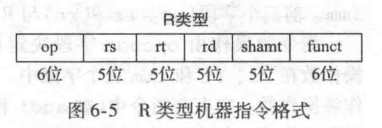
\includegraphics[width =0.9 \linewidth]{figure/Rtype.png}

32位指令分为6个字段:op、rs、rt、rd、shamt和funct。指令的操作编码由op和funct决定,R类型指令的op操作码都是0,故特定R类型操作由funct字段决定。指令的操作数编码包括3个字段:rs、rt和rd。前两个寄存器rs和rt是源寄存器,rd是目的寄存器。shamt字段仅仅用于移位操作,其中数值表示移位的位数,对于其他R类型指令,shamt为0。

在本次实验中,我们实现的R类型指令包括:

\begin{itemize}
\item {\bf nop:} 空指令,不做任何操作。其op字段编码为全0,因此被归类于R类型指令,等价于指令sll \$r0, \$r0, \$r0。
\item {\bf add, sub, and, or, slt:} 运算指令,将寄存器rs与rt中的值运算后,写入rd寄存器。五种运算分别为:[rs] + [rt], [rs] - [rt], [rs] \& [rt], [rs] | [rt], ([rs] < [rt])?1:0。
\item {\bf sll, sra, srl:} 移位指令,将寄存器rt中的值(左/右)移shamt位后,写入rd寄存器。默认rs字段为0。三种移位分别为:左移(补0),算术右移(补符号位),逻辑右移(补0)。
\item {\bf jr:} 跳转寄存器指令,跳至寄存器rs中的值所在的地址。默认rt、rd字段为0。因为涉及寄存器PC的更改,所以被归类于R类型指令。
\end{itemize}

{\color{red} 后四条指令为补充指令!}

\subsubsection{I型指令}

I类型是{\em 立即数类型}的缩写。I类型指令有两个寄存器操作数和一个立即数操作数。下图给出了I类型机器指令格式:

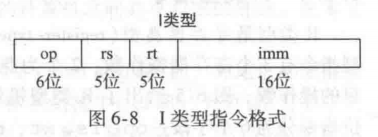
\includegraphics[width =0.9 \linewidth]{figure/Itype.png}

一条32位指令有4个字段:op、rs、rt和imm。前三个字段与R类型指令一样。imm字段代表一个16位立即数。指令的操作由opcode字段决定。操作数在rs、rt和imm三个字段中。rs和imm常用于源操作数。rt既可用于目的操作数,也可用于源操作数。

在本次实验中,我们实现的I类型指令包括:

\begin{itemize}
\item {\bf addi, andi, ori, slti:} 运算指令,将寄存器rs中的值与立即数imm运算后,写入rt寄存器。四种运算分别为:[rs] + imm, [rs] \& imm, [rs] | imm, ([rs] < imm) ? 1 : 0。
\item {\bf sw, lw:} 存取指令,从内存某地址处读取(向内存某地址处写入)寄存器rt中的值。内存器地址的计算方式为:[rs] + imm
\item {\bf beq, bne:} 条件转移指令。当寄存器rs与rt中的值相等(不等)时,跳至某地址处。跳转地址的计算方式为:PC + 4 + (imm << 2)
\end{itemize}

\subsubsection{J型指令}

J类型是{\em 跳转类型}的缩写。这种格式仅用于跳转指令。下图给出了J类型机器指令格式:

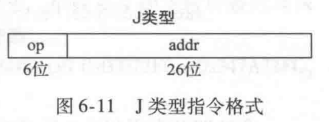
\includegraphics[width =0.9 \linewidth]{figure/Jtype.png}

这种指令格式有一个26位地址操作数addr。与其他格式一样,J类型指令由一个6位opcode开始,决定操作类型。剩下的位用于指定地址addr。

\begin{itemize}
\item {\bf j:} 跳转指令,直接跳至某地址处。地址的计算方式为:\{PC + $\textit{4}_{31..28}$, addr, 00\}。
\item {\bf jal:} 跳转写入指令,跳至某地址处,并将当前PC值写入\$ra寄存器。地址的计算方式为:\{PC + $\textit{4}_{31..28}$, addr, 00\}。
\end{itemize}

{\color{red} jal指令为补充指令!}

\subsection{{\color{red} MIPS汇编器实现}}

为了更方便的书写测试代码,我特地使用Python写了一个MIPS指令的汇编器,将汇编代码翻译为机器代码。

汇编器的设计思路如下:
\begin{enumerate}
\item 扫描整个文件,处理出label对应的地址。
\item 依次处理每条指令,因为指令长度固定,所以每次可以让PC值直接加四。
\item 将指令分为三种类型,三种类型分别对应三种译码方式。
\item 若为R类型或I类型指令,则利用字符串处理从中分离出寄存器,译码后放入对应位置。
\item 若为I类型或J类型指令,则从指令中提取立即数,注意立即数可以以label的形式给出。
\item 在计算地址时,需注意I类型指令为相对寻址(相对于PC+4),J类型指令则为直接寻址(高四位与PC+4相同,低两位为0)。
\end{enumerate}

最终的输出格式有两种:一种是.out文件,便于阅读;另一种是.txt文件,可用于直接写入Imem。

%\newpage
\section{部件分析}

\subsection{多路复用器MUX2}

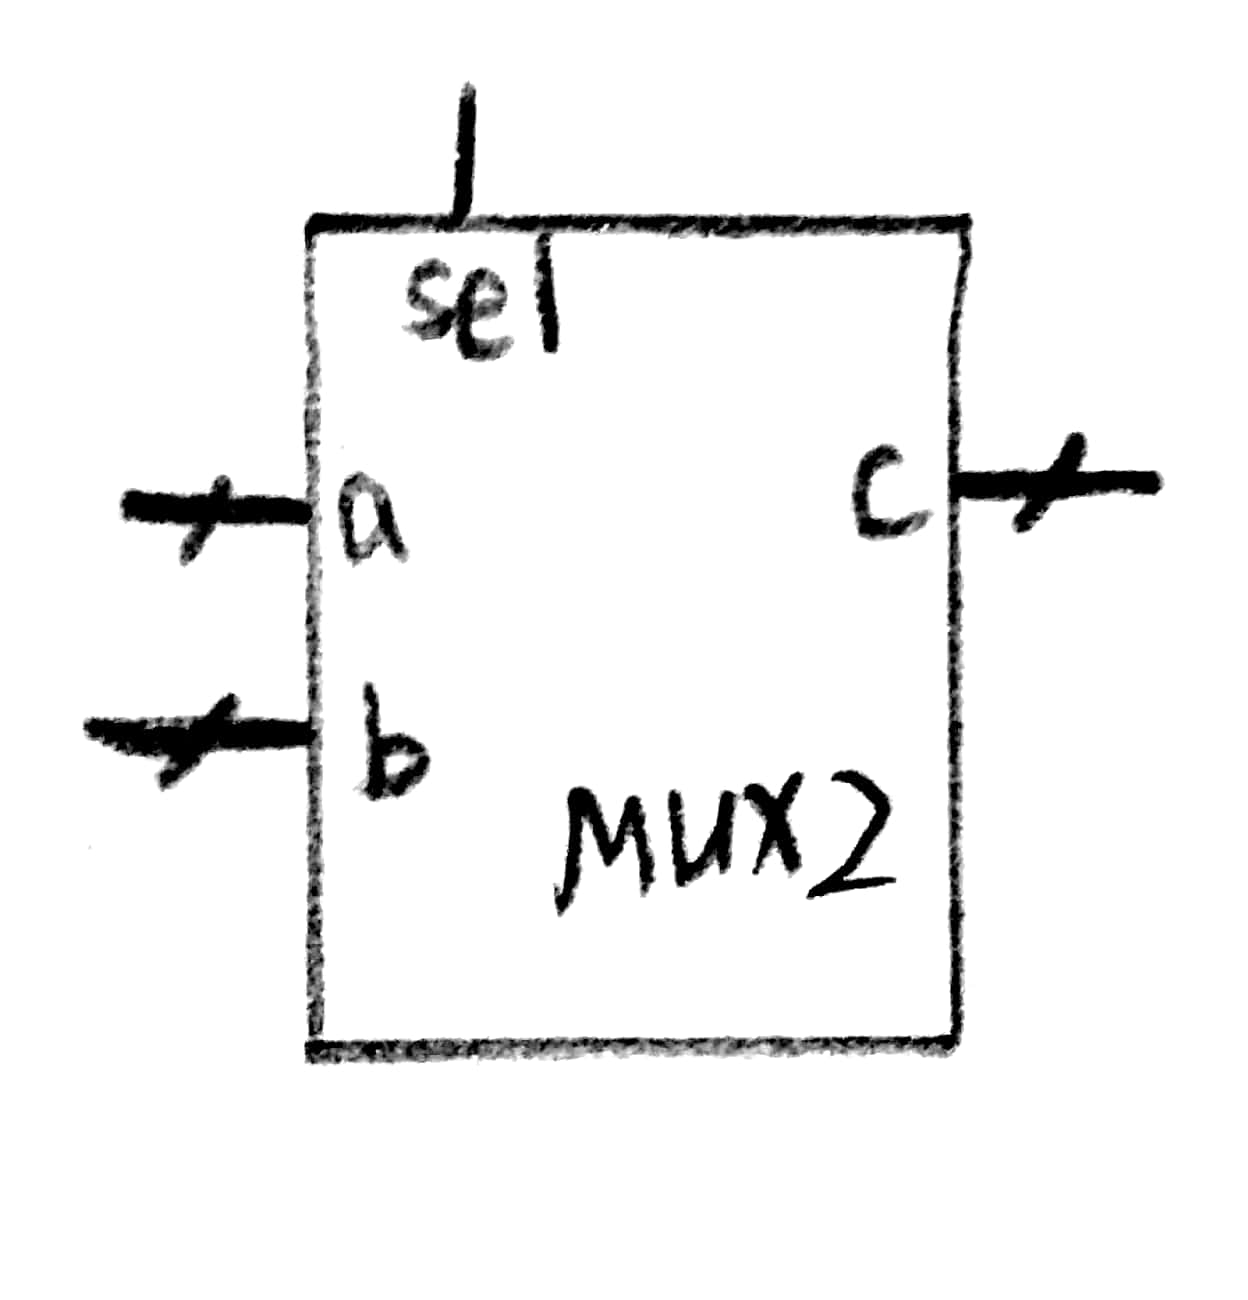
\includegraphics[width =0.25 \linewidth]{figure/MUX2.jpg}

{\bf 功能说明:} 操作数长度可选的多路复用器。当sel = 0时,c = a;当sel = 1时,c = b。

{\bf 实现细节:} 在模块时引入参数parameter定义操作数长度,利用assign语句搭配(sel == 0)?a:b做选择。

\subsection{加法器Adder}

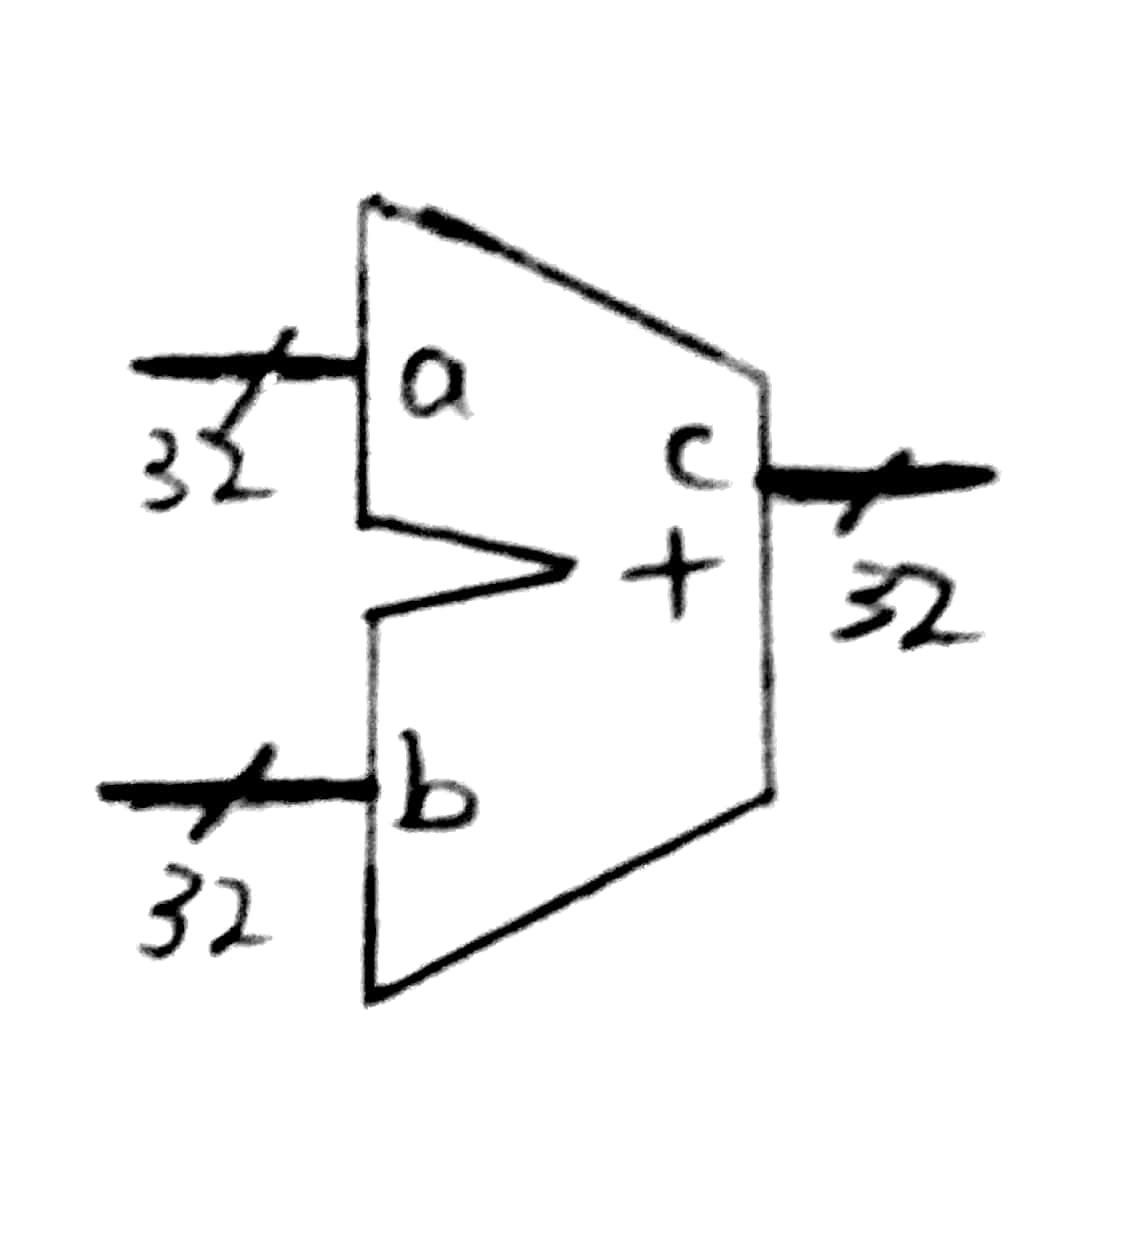
\includegraphics[width =0.25 \linewidth]{figure/Adder.jpg}

{\bf 功能说明:} 32位加法器,c = a + b,用于计算PC值与跳转地址。

{\bf 实现细节:} 通过assign语句和Verilog自带的加法器实现。

\subsection{移位器SL2}

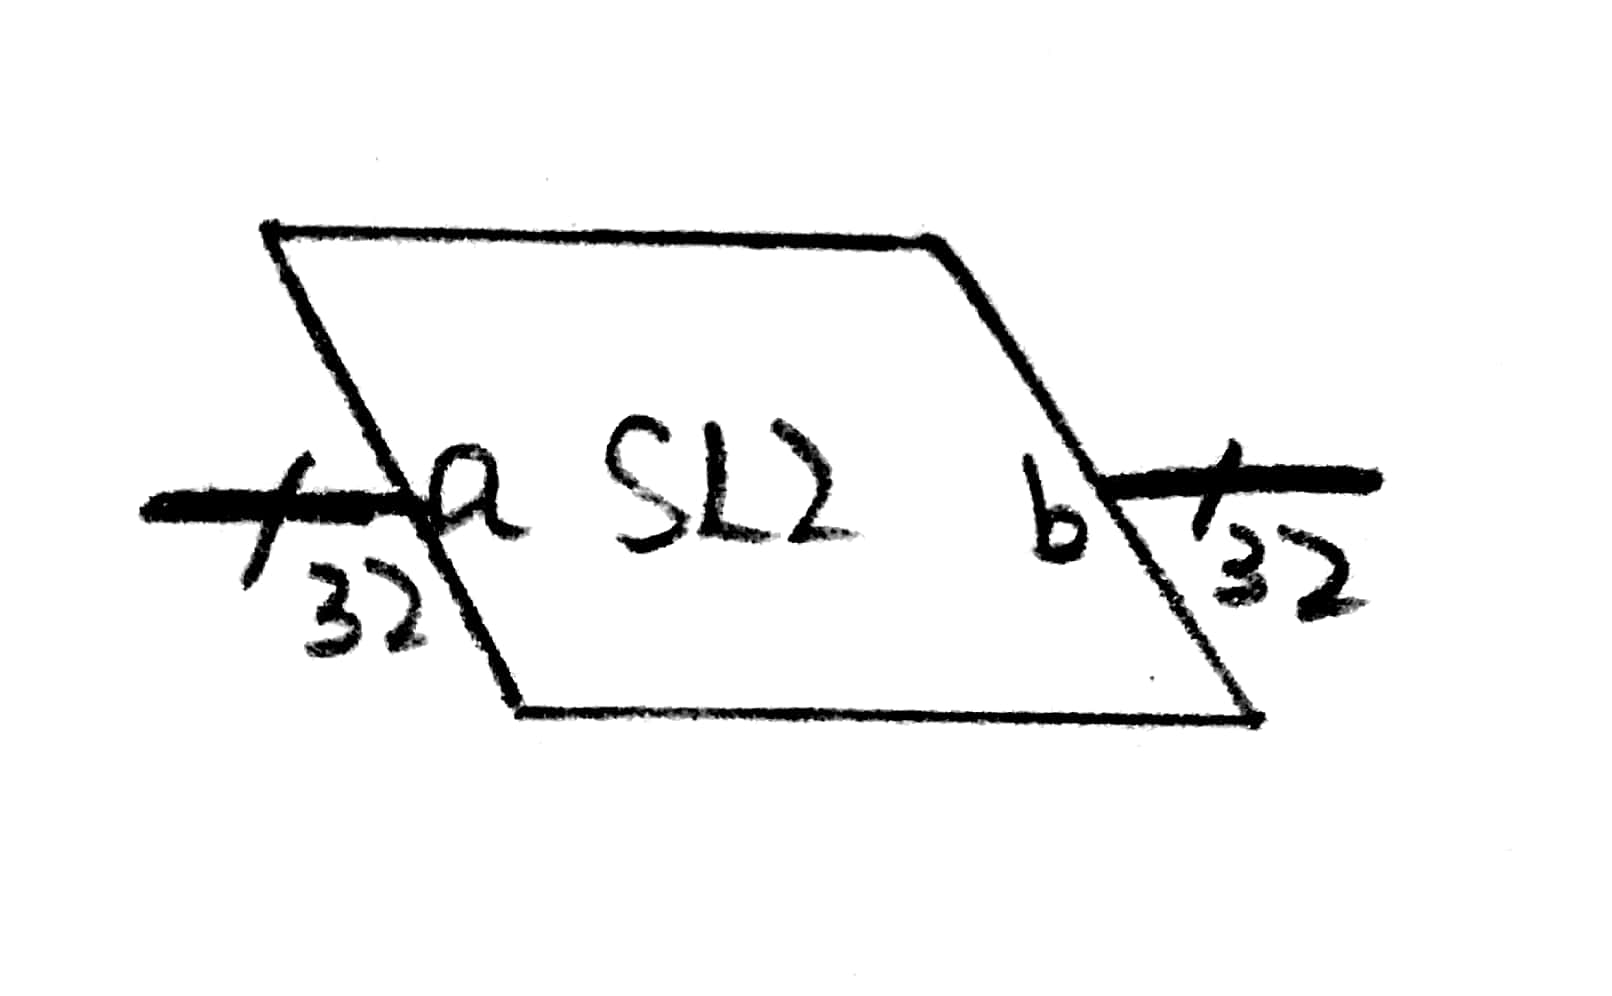
\includegraphics[width =0.25 \linewidth]{figure/SL2.jpg}

{\bf 功能说明:} 将32位数左移2位, b = a << 2,用于立即数的字对齐。 

{\bf 实现细节:} 通过assign语句和拼接操作实现。

\subsection{位扩展SignExtend}

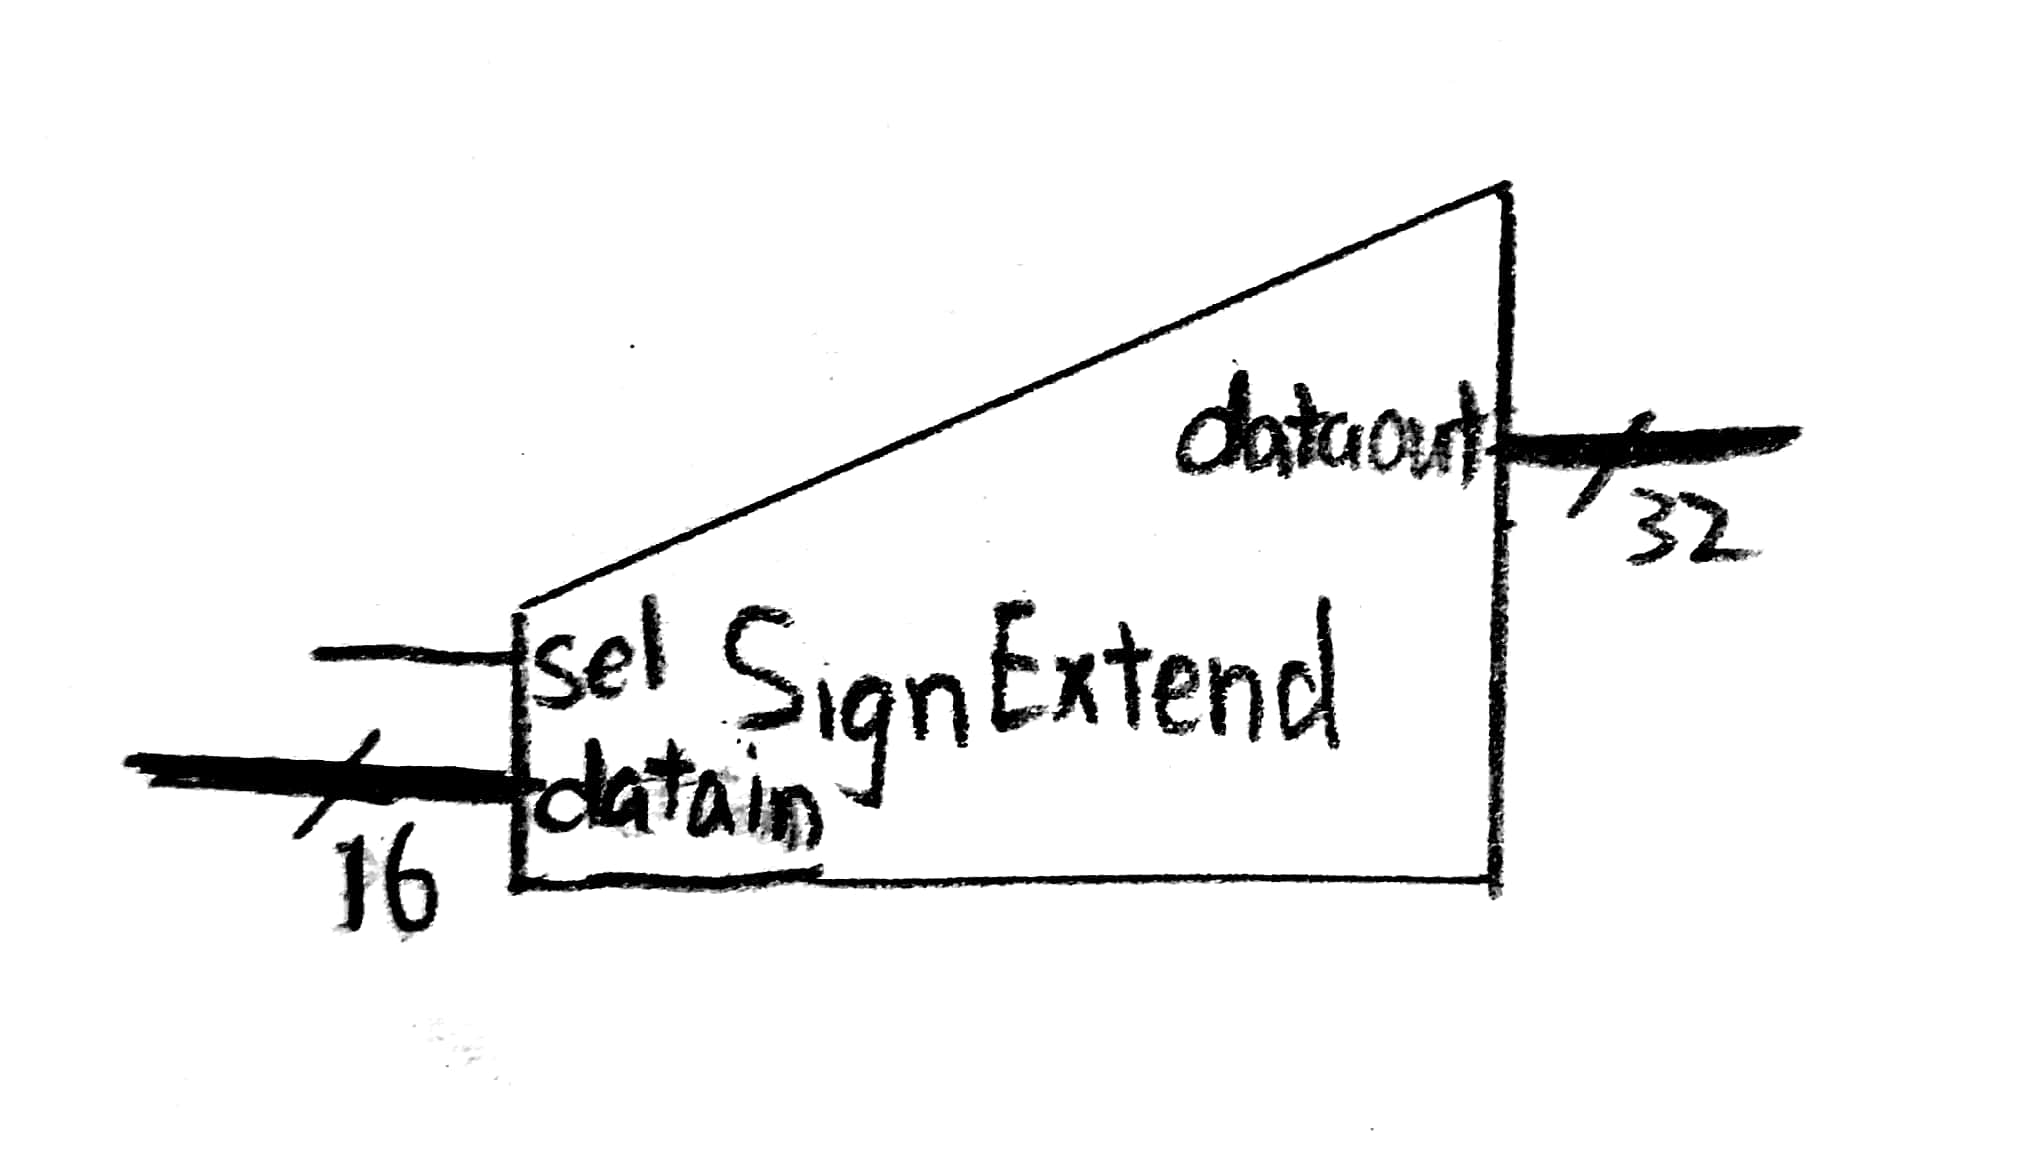
\includegraphics[width =0.35 \linewidth]{figure/SignExtend.jpg}

{\bf 功能说明:} 将16位数扩展为32位数。当sel = 0时,进行符号扩展;当sel = 1时,进行0扩展。用于扩展指令中的16位立即数。

{\bf 实现细节:} 利用assign语句和拼接操作。

\subsection{触发器flopr}

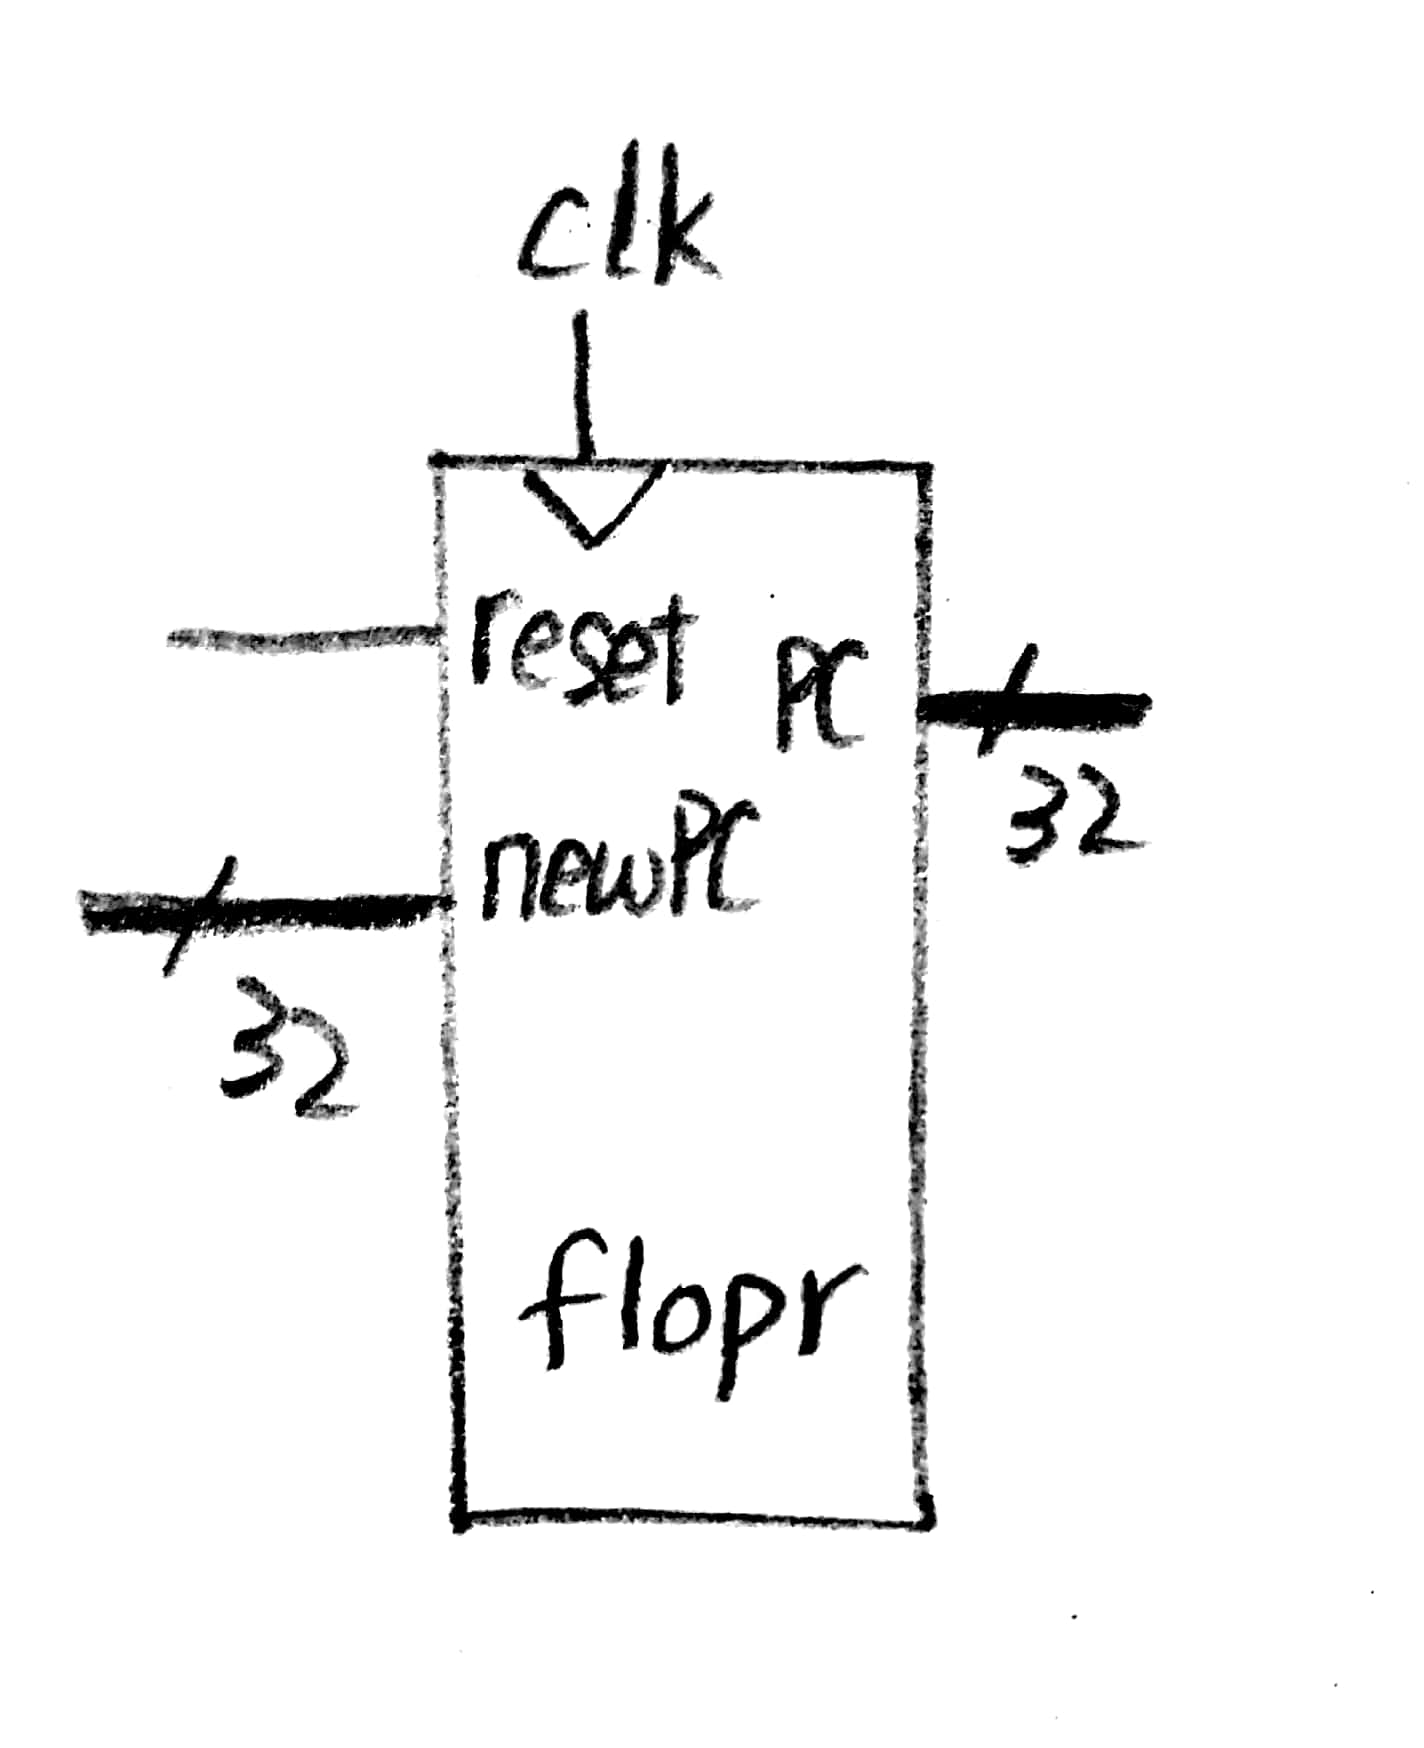
\includegraphics[width =0.25 \linewidth]{figure/flopr.jpg}

{\bf 功能说明:} 32位触发器。当clk到达上升沿时,将newPC的值写入PC;当reset = 1时,将PC清零。用于存储PC。

{\bf 实现细节:} 简单的always模块,reset设置为同步清零端。

\subsection{算术逻辑单元ALU}

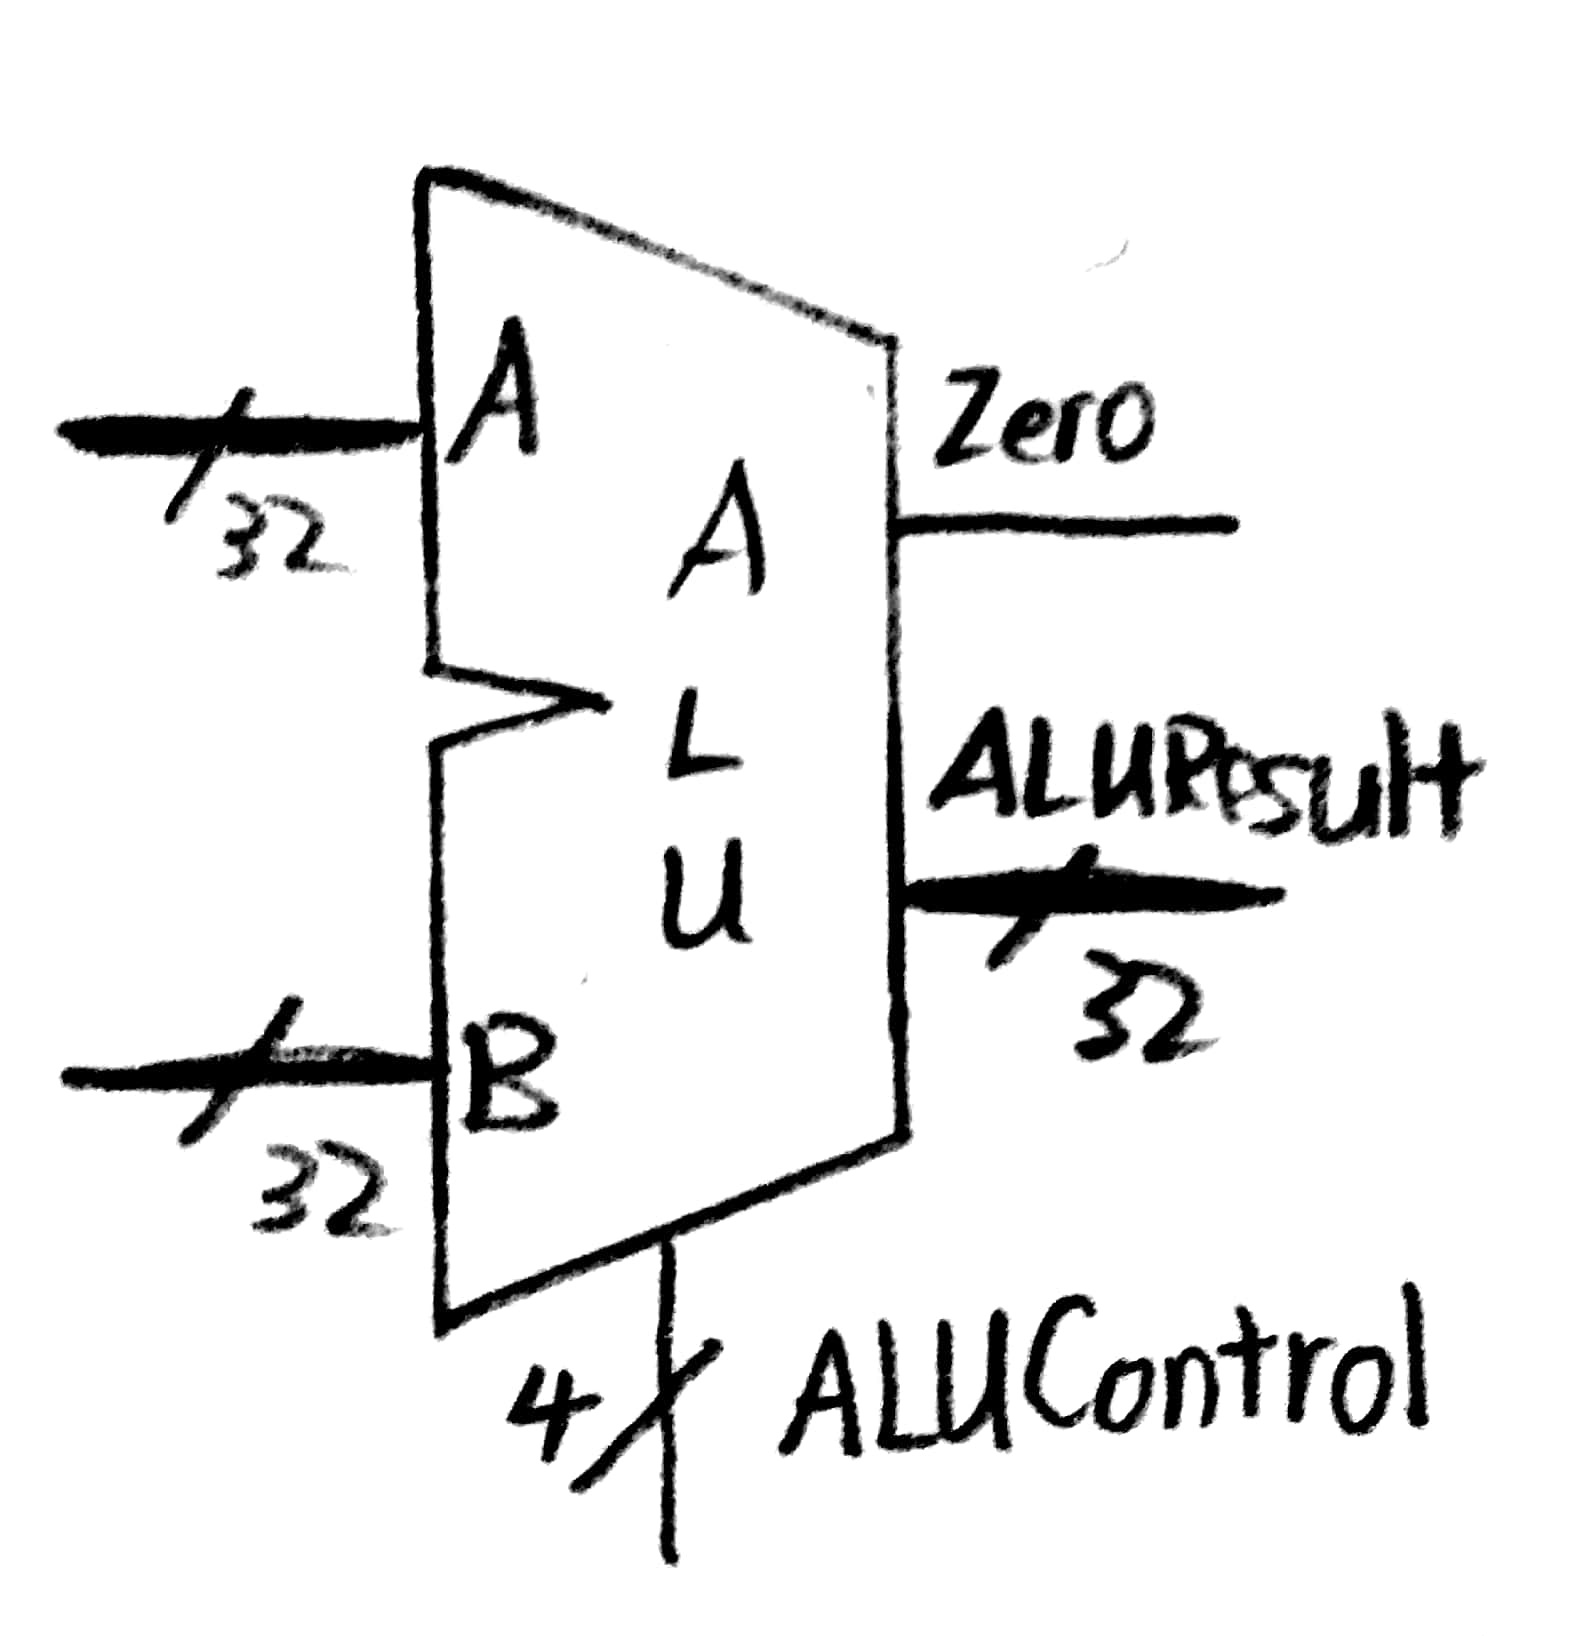
\includegraphics[width =0.3 \linewidth]{figure/ALU.jpg}

{\bf 功能说明:} 根据ALUControl信号,进行运算,zero信号为零标志。运算表如下:
% Please add the following required packages to your document preamble:
% \usepackage[table,xcdraw]{xcolor}
% If you use beamer only pass "xcolor=table" option, i.e. \documentclass[xcolor=table]{beamer}
\begin{table}[htbp]
\begin{tabular}{
>{\columncolor[HTML]{C0C0C0}}c 
>{\columncolor[HTML]{EFEFEF}}c 
>{\columncolor[HTML]{C0C0C0}}c 
>{\columncolor[HTML]{EFEFEF}}c }
ALUControl                   & ALUResult                            & ALUControl                   & ALUResult                                                                                                     \\
\cellcolor[HTML]{EFEFEF}0000 & \cellcolor[HTML]{C0C0C0}A \& B       & \cellcolor[HTML]{EFEFEF}0101 & \cellcolor[HTML]{C0C0C0}A | $\sim$B                                                                           \\
0001                         & A | B                                & 0110                         & A - B                                                                                                         \\
\cellcolor[HTML]{EFEFEF}0010 & \cellcolor[HTML]{C0C0C0}A + B        & \cellcolor[HTML]{EFEFEF}0111 & \cellcolor[HTML]{C0C0C0}(A\textless{}B)?1:0                                                                   \\
0011                         & B \textless{}\textless A             & 1000                         & \begin{tabular}[c]{@{}c@{}}B\textgreater{}\textgreater{}A\\ (logic)\end{tabular}                              \\
\cellcolor[HTML]{EFEFEF}0100 & \cellcolor[HTML]{C0C0C0}A \& $\sim$B & \cellcolor[HTML]{EFEFEF}1001 & \cellcolor[HTML]{C0C0C0}\begin{tabular}[c]{@{}c@{}}B\textgreater{}\textgreater{}A\\ (arithmetic)\end{tabular}
\end{tabular}
\caption{ALU功能表}
\end{table}

{\bf 实现细节:} 使用case语句对ALUControl信号进行判断,然后用Verilog内置的运算单元进行运算。最后通过assisng语句判断ALUResult是否为0,设置zero信号。

\subsection{指令存储器Imem}

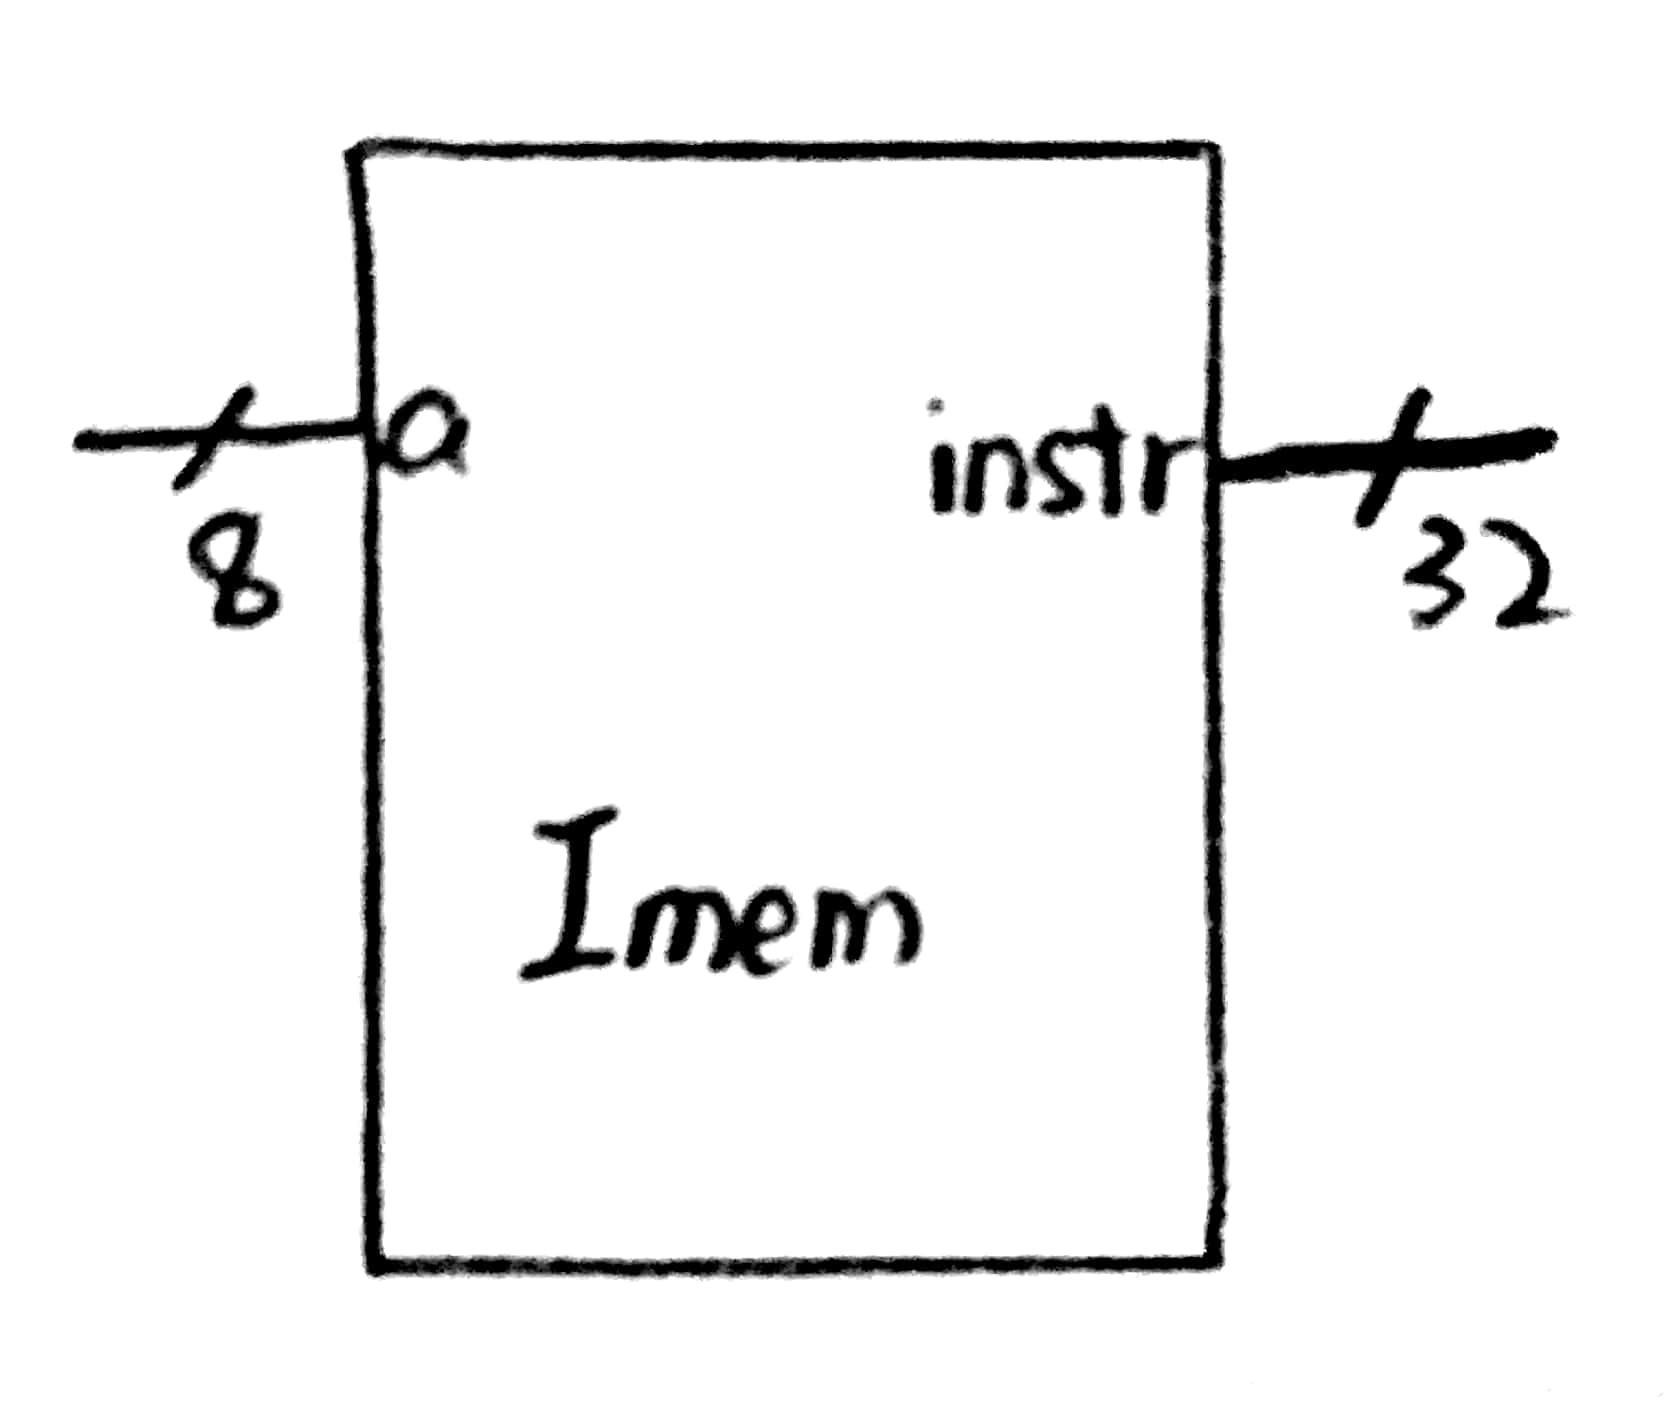
\includegraphics[width =0.3 \linewidth]{figure/Imem.jpg}

{\bf 功能说明:} 指令存储器。根据8位地址a读取指令instr。

{\bf 实现细节:} 定义256个长度为8的寄存器。\footnote{与课本中的写法不同,这里我们按照实际机器中每个寄存器对应一个字节(8 bits)的方式开数组} 注意定义时二维数组的两维不能搞反,前面一维表示寄存器的长度,后面一维表示寄存器的个数。
\begin{lstlisting}[language=Verilog]  
reg [7:0] RAM[255:0]; 
\end{lstlisting}  
初始化时,利用initial将预先写好的机器编码写入RAM寄存器。写的时候,因为实际指令的长度为32,所以我们需要一次写四个寄存器。
\begin{lstlisting}[language=Verilog]  
initial
    begin
    {RAM[3], RAM[2], RAM[1], RAM[0]} <= 32'h20080063;
    {RAM[7], RAM[6], RAM[5], RAM[4]} <= 32'h20090025;
    end
\end{lstlisting}  
用assign语句读取a地址对应的指令编码,注意一次要读四个寄存器。
\begin{lstlisting}[language=Verilog]  
assign instr = {RAM[a+3],RAM[a+2],RAM[a+1],RAM[a]};
\end{lstlisting}  
读要写成组合逻辑!

\subsection{数据存储器Dmem}

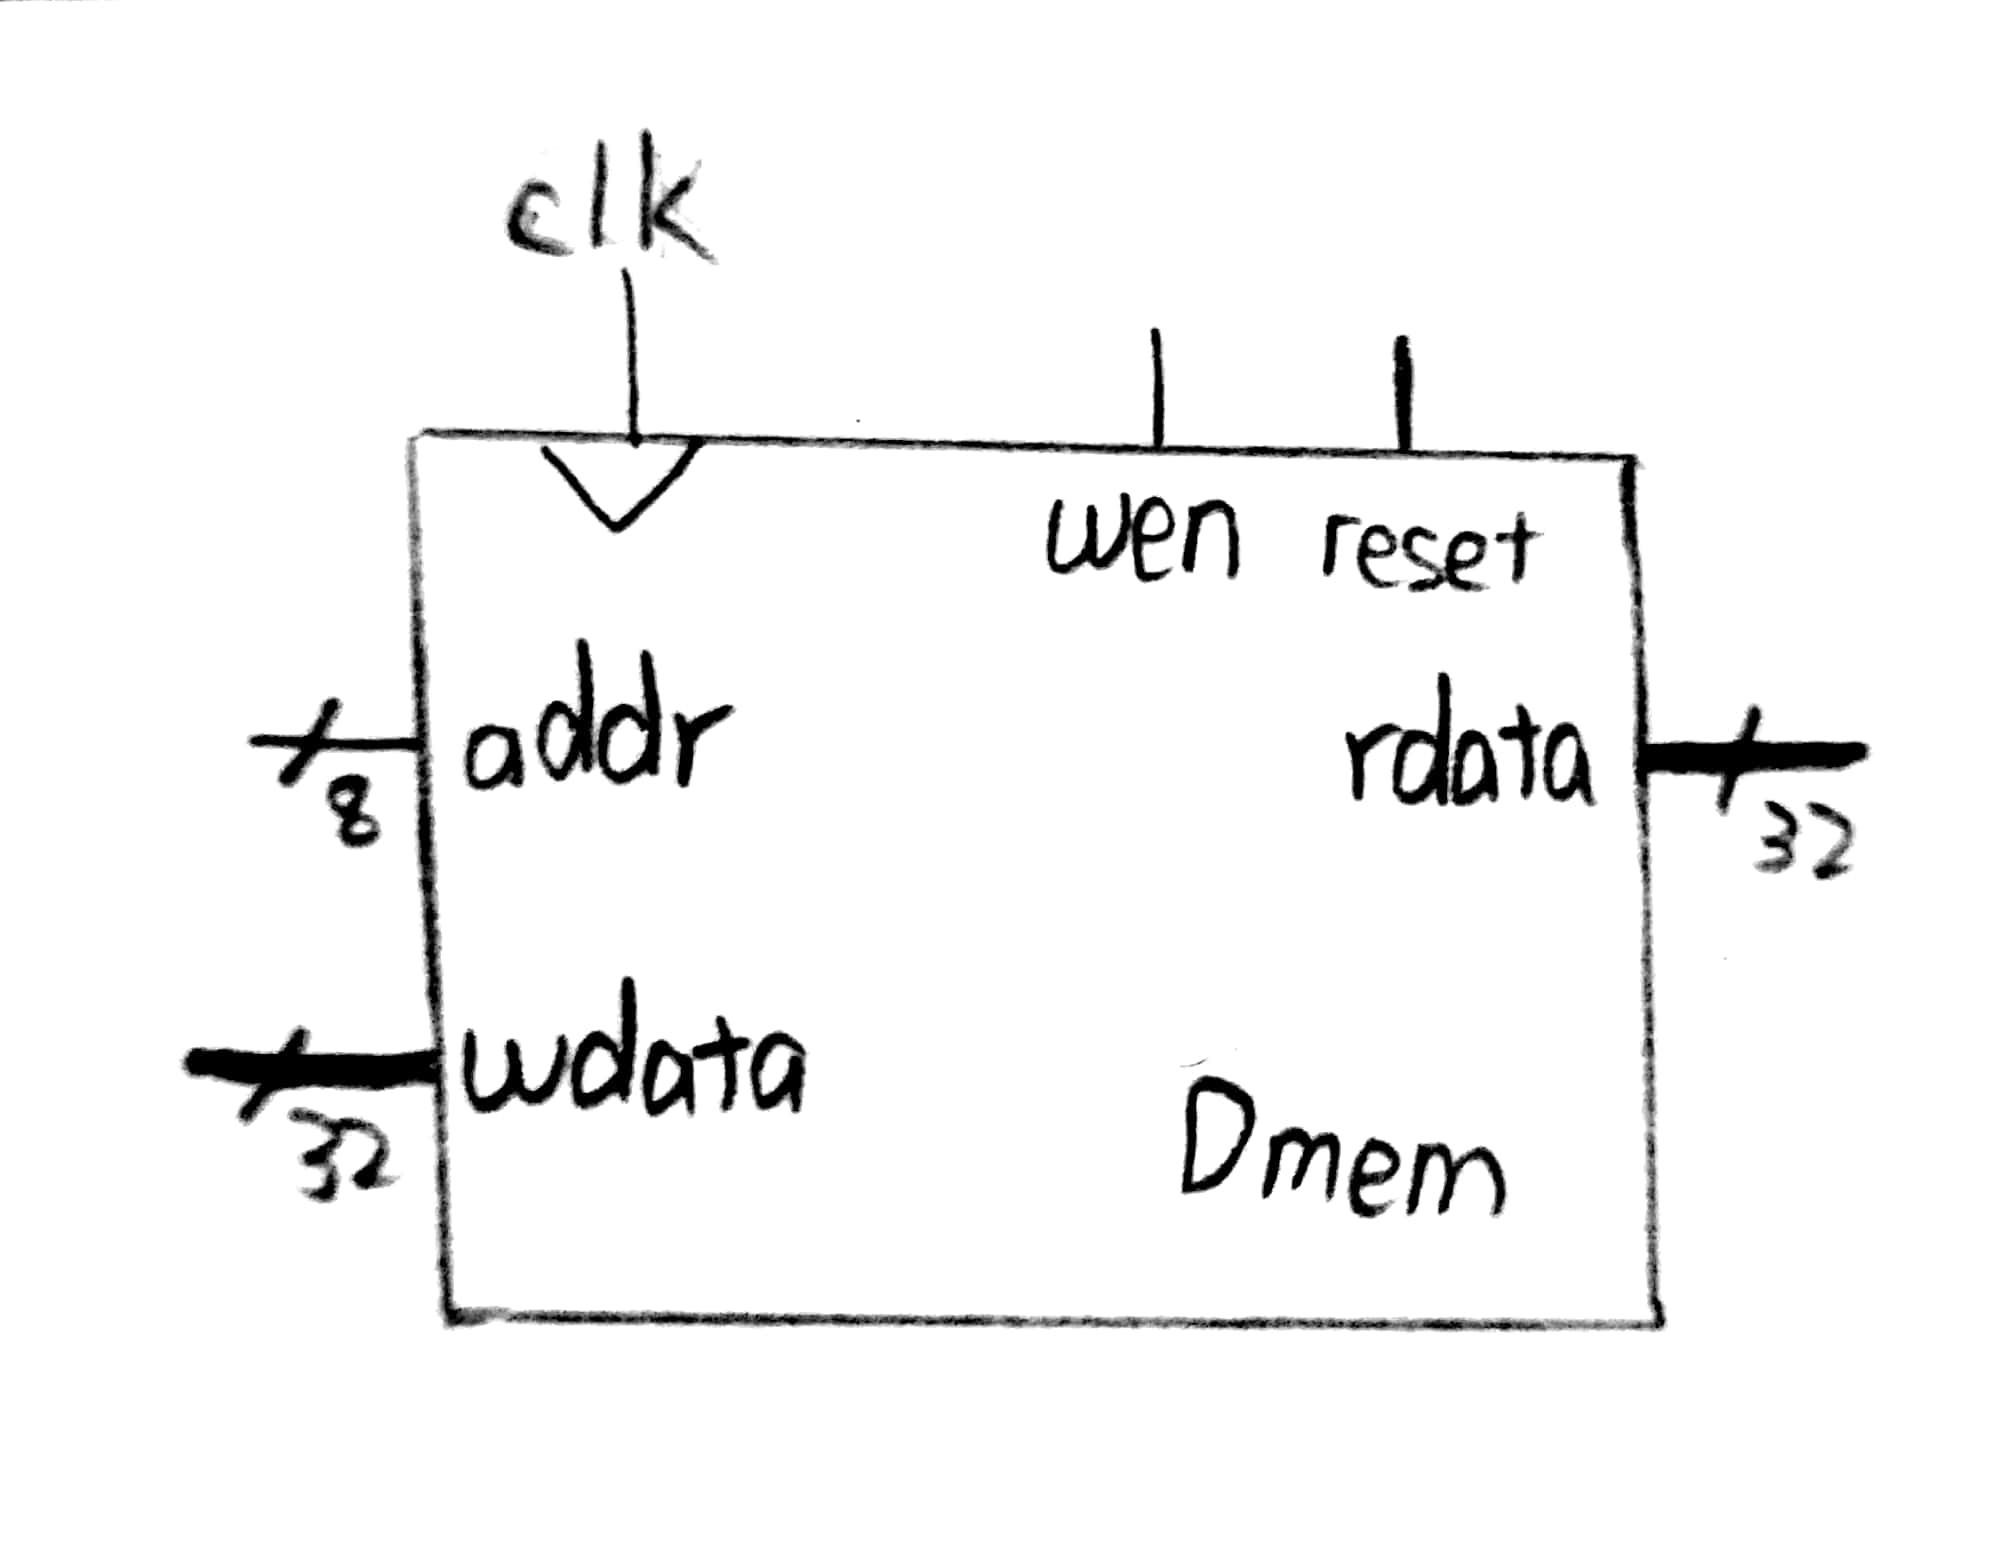
\includegraphics[width =0.3 \linewidth]{figure/Dmem.jpg}

{\bf 功能说明:} 数据存储器。当reset = 1时,将内存中全部数据清零;否则,当wen = 1时,向addr地址写入wdata。rdata始终等于addr地址处的值。

{\bf 实现细节:} 原理同Imem。当reset为1时,可利用for语句对RAM进行清零。
\begin{lstlisting}[language=Verilog]  
if (reset)
      begin
        for (j = 0; j < 32; j = j + 1) 
            RAM[j] <= 0;
      end
\end{lstlisting}  
写入时,同样要同时写四个寄存器。
\begin{lstlisting}[language=Verilog]  
if (wen) RAM[addr+3], RAM[addr+2], RAM[addr+1], RAM[addr]} <= wdata;
\end{lstlisting} 

\subsection{寄存器文件RegFile}

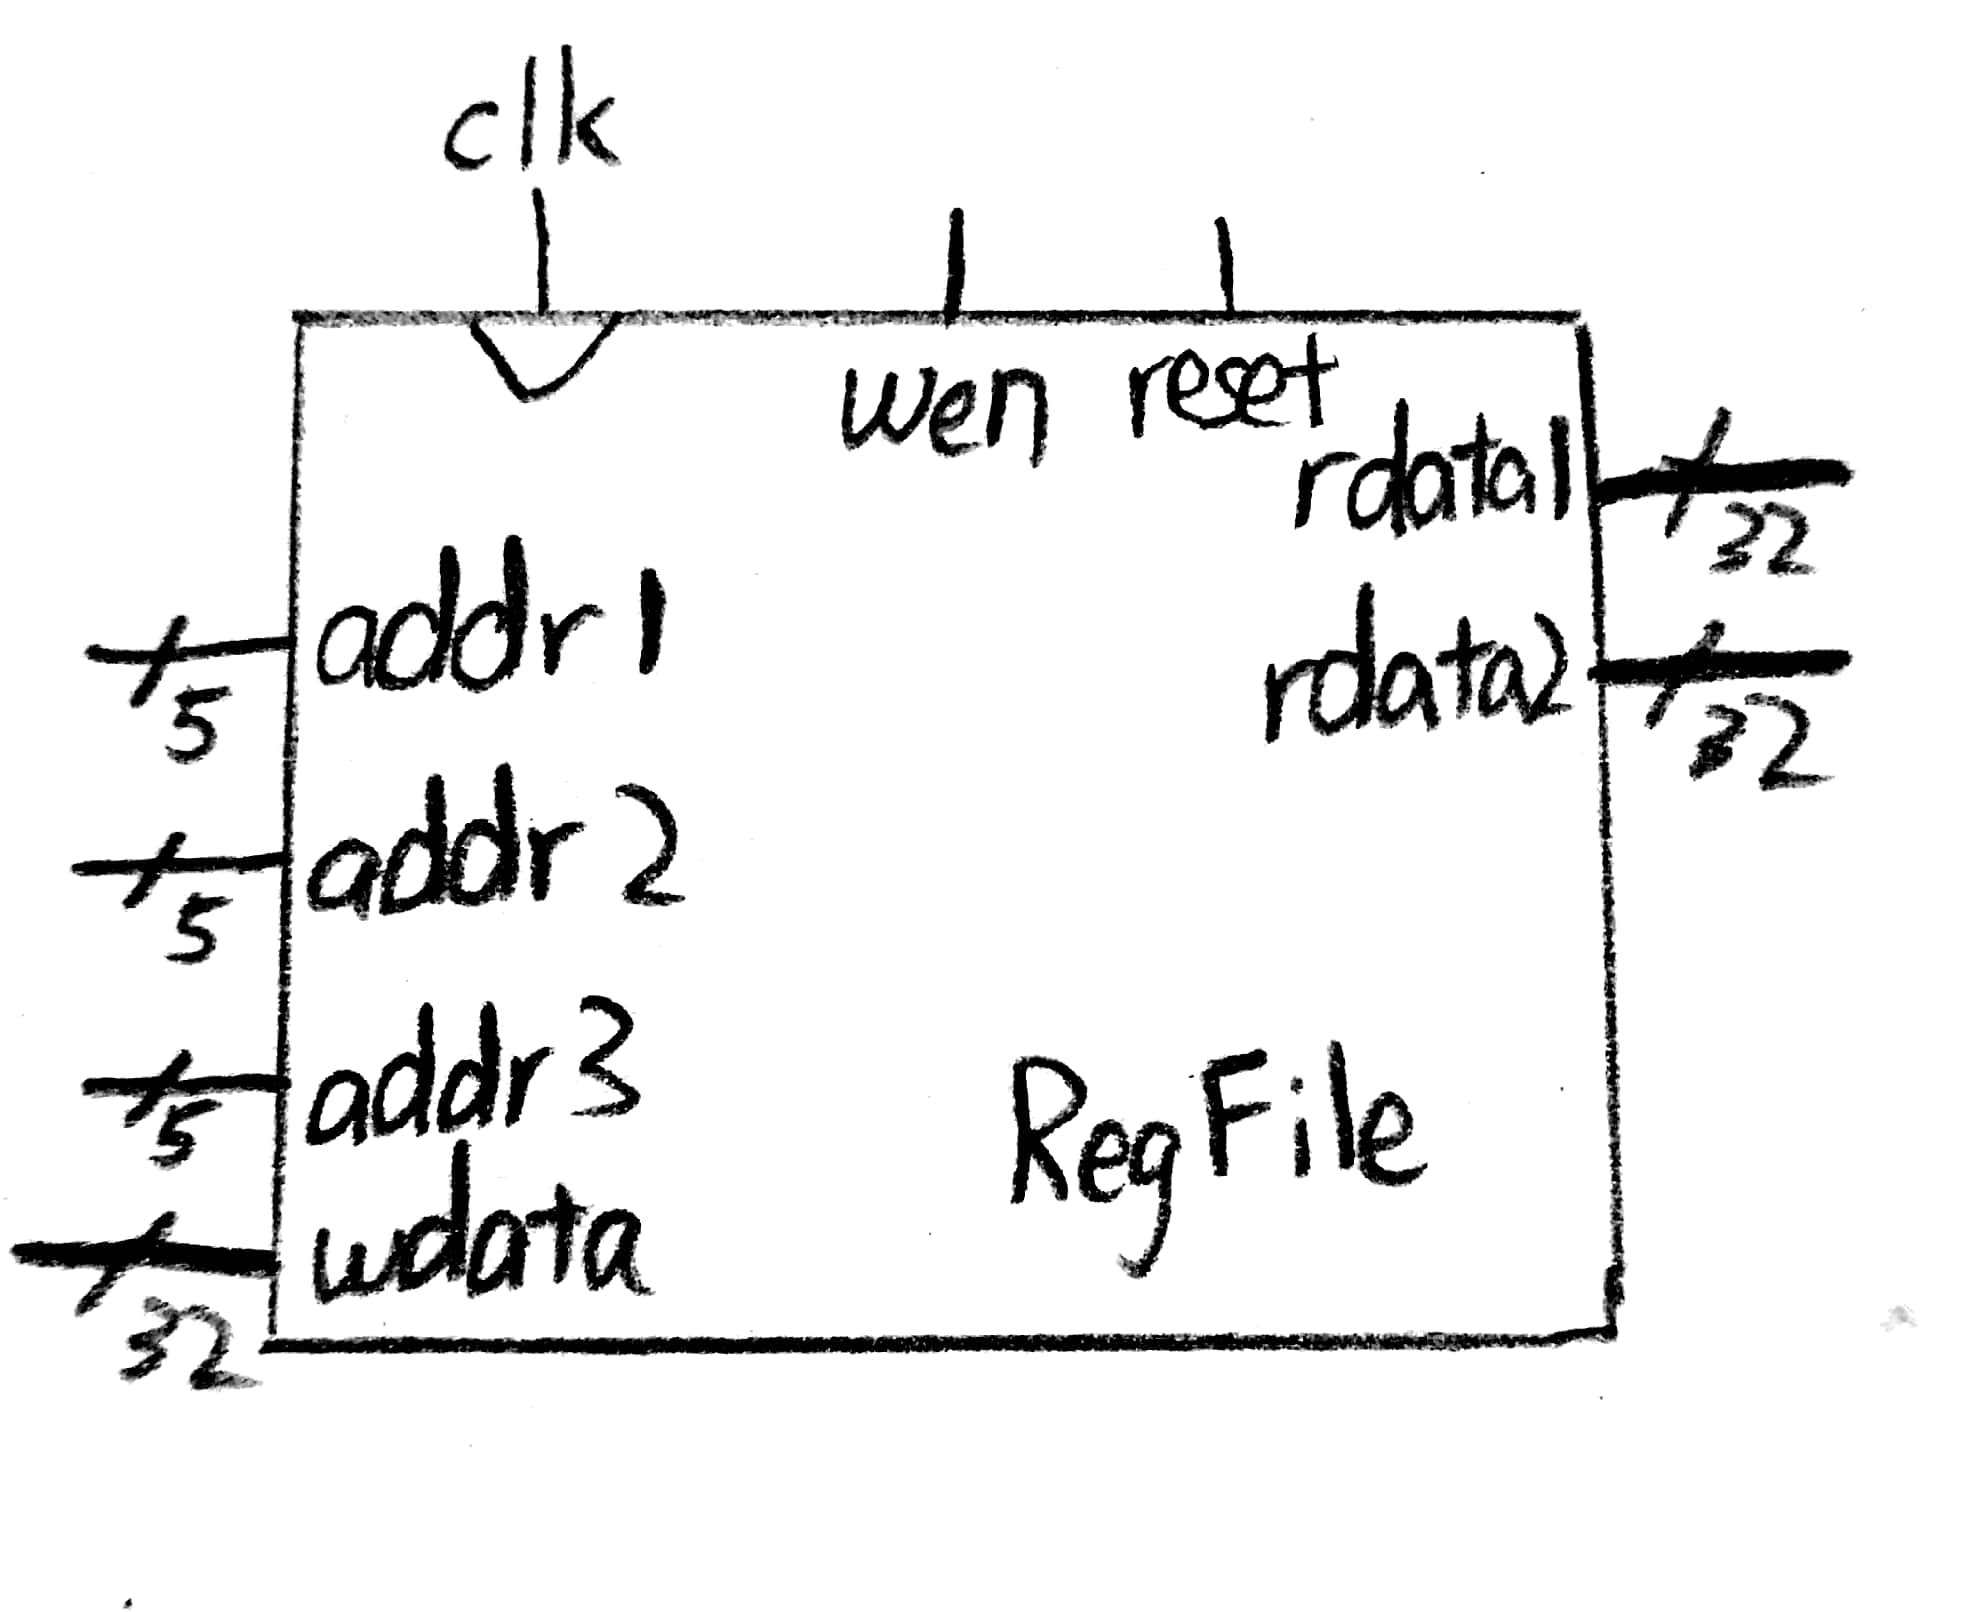
\includegraphics[width =0.3 \linewidth]{figure/Regfile.jpg}

{\bf 功能说明:} 寄存器文件。从addr1与addr2两个寄存器同时读数据,结果放入rdata1和rdata2中;当reset=1时,将所有寄存器中的数据清零;否则,当wen=1时,向addr3寄存器写入数据wdata。

{\bf 实现细节:} 原理同Dmem。要注意0号寄存器的值始终为0,所以我们直接判断若addr=0,则直接返回0。
\begin{lstlisting}[language=Verilog]  
assign rdata1 = (addr1 != 0) ? rf[addr1] : 0;
assign rdata2 = (addr2 != 0) ? rf[addr2] : 0;
\end{lstlisting} 

\begin{figure*}[htbp]
\centering
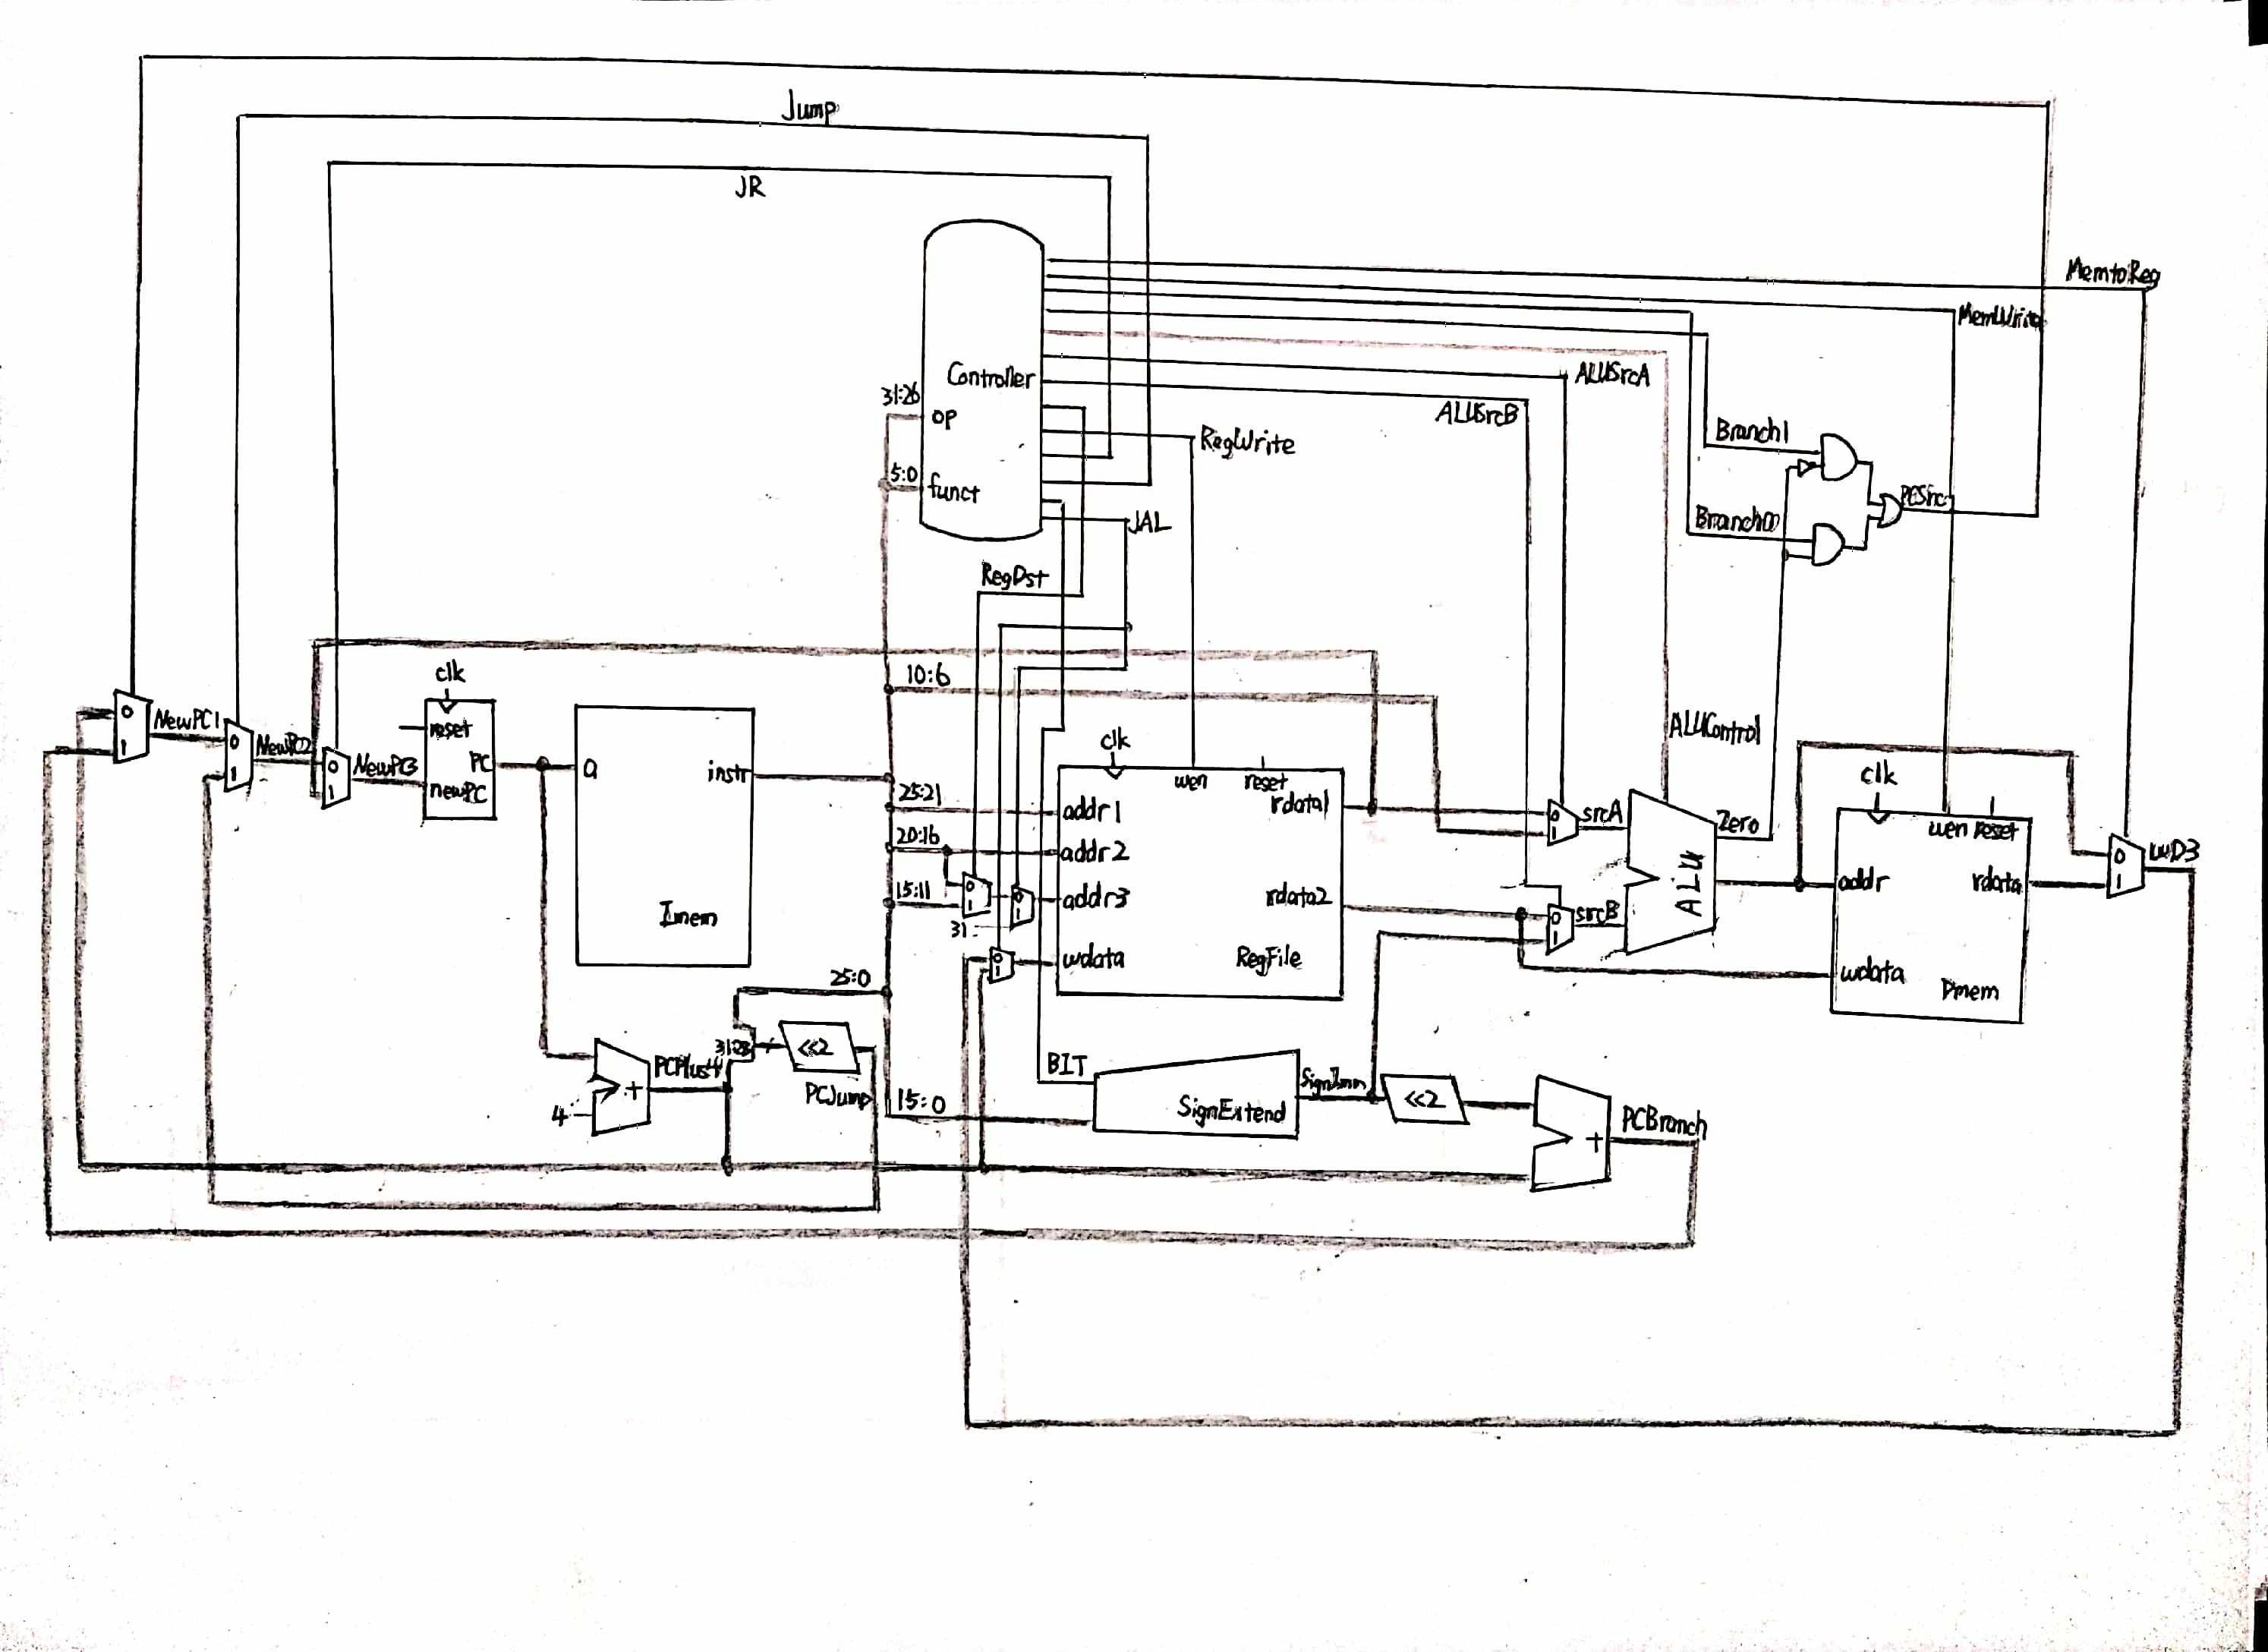
\includegraphics[width = 0.8\linewidth]{figure/datapath.jpg}
\caption{数据通路Datapath}
\label{fig:datapath}
\end{figure*}

\subsection{数据通路Datapath}

整个数据通路连接如图~\ref{fig:datapath}所示,因为新添加了几条指令,所以与课本中的通路略有不同。

{\bf 功能说明:} 连接所有元件,传递信号。从左至右依次解释如下:
\begin{itemize}
\item 最左侧为三个二路选择器\footnote{因为指令是一条一条添加的,所以多路器也是一个一个添加的,也可以仅用一个多路器实现。},用于选择新的PC值。
\begin{enumerate}
\item 用于分支指令beq和bne,选择信号为PCSrc。当PCSrc = 0时,正常递增,选择PC+4的值;当PCSrc = 1时,选择分支地址PCBranch。
\item 用于直接跳转指令j和jal,选择信号为Jump。当Jump = 0时,不直接跳转,选择NewPC1;当Jump = 1时,选择直接跳转地址PCJump。
\item 用于寄存器跳转指令jr,选择信号为JR。当JR = 0时,不发生寄存器跳转,选择NewPC2;当 JR = 1时,将从寄存器中读出的值RD1作为跳转地址。
\end{enumerate}
因此,新的PC值共有四个来源:正常递增PC+4,分支跳转PCBranch,直接跳转PCJump,寄存器跳转RD1。
\item 将PC值作为Imem的输入地址,读出的instr相应位传入RegFile,读取相应的寄存器值。
\item 左下方先用加法器计算PC+4的值,结果记为PCPlus4;再将PCPlus的高4位与instr的后26位拼接,左移两位后,作为直接跳转的地址PCJump。
\item 寄存器文件的写使能由RegWrite信号控制,写入的寄存器有三种情况:当指令为R类型时,RegDst = 1,选择指令中的rd字段作为目的寄存器;当指令为I类型时,RegDst = 0,选择指令中的rt字段作为目的寄存器;当指令为jal时,目的寄存器为\$ra。两个多路器分别由信号RegDst、JAL控制。写入数据有三种选择:当指令为lw时,MemtoReg = 1,选择从内存中读取的值;当指令为jal时,JAL = 1,将PCPlus4的值写入寄存器\$ra;否则,选择运算结果ALUResult作为写入数据。
\item 中间下方由扩展器,移位器和加法器组成。扩展器可根据BIT信号选择符号扩展或按0扩展。左移两位后与PCPlus4相加,结果作为相对寻址的地址PCBranch。
\item ALU的功能选择信号为四位信号ALUControl,两个运算数分别为SrcA与SrcB。SrcA可选择寄存器文件RD1的值,也可以是指令中shamt字段的值,后者用于移位操作。SrcB可选择寄存器文件RD2的值,也可以是立即数扩展后的值,后者主要用于I类型指令。两个多路器的选择信号分别为ALUSrcA与ALUSrcB。
\item Dmem始终将ALUResult作为读写的地址,RD2作为写入的数据,写使能由信号MemWrite控制。
\item 当指令为beq且零标志为1或指令为bne且零标志为0时,分支指令的信号PCSrc = 1,进行分支跳转。
\end{itemize}

{\bf 实现细节:} 我在实现时并未单独开一个datapath模块,而是选择直接在顶层模块中连接电路。为了便于检查元件位置与数量,我在书写代码的时候是按照图中从左至右的顺序进行书写的。



\subsection{控制模块Controller}
\label{sec:controller}

\begin{table*}[t]
\begin{tabular}{cccccccccccccccc}
\hline
\multicolumn{1}{c}{opcode} & \multicolumn{1}{c}{funct} & \multicolumn{1}{c}{} & \multicolumn{1}{c}{RW} & \multicolumn{1}{c}{RD} & \multicolumn{1}{c}{SA} & \multicolumn{1}{c}{SB} & \multicolumn{1}{c}{B0} & \multicolumn{1}{c}{B1} & \multicolumn{1}{c}{MW} & \multicolumn{1}{c}{MR} & \multicolumn{1}{c}{JR} & \multicolumn{1}{c}{J} & \multicolumn{1}{c}{JAL} & \multicolumn{1}{c}{BIT} & aluop \\ \hline
000000                      & 100000                     & add                   & 1                       & 1                       & 0                       & 0                       & 0                       & 0                       & 0                       & 0                       & 0                       & 0                      & 0                        & 0                        & 010   \\
000000                      & 100010                     & sub                   & 1                       & 1                       & 0                       & 0                       & 0                       & 0                       & 0                       & 0                       & 0                       & 0                      & 0                        & 0                        & 010   \\
000000                      & 100100                     & and                   & 1                       & 1                       & 0                       & 0                       & 0                       & 0                       & 0                       & 0                       & 0                       & 0                      & 0                        & 0                        & 010   \\
000000                      & 100101                     & or                    & 1                       & 1                       & 0                       & 0                       & 0                       & 0                       & 0                       & 0                       & 0                       & 0                      & 0                        & 0                        & 010   \\
000000                      & 101010                     & slt                   & 1                       & 1                       & 0                       & 0                       & 0                       & 0                       & 0                       & 0                       & 0                       & 0                      & 0                        & 0                        & 010   \\
001000                      &                            & addi                  & 1                       & 0                       & 0                       & 1                       & 0                       & 0                       & 0                       & 0                       & 0                       & 0                      & 0                        & 0                        & 000   \\
001100                      &                            & andi                  & 1                       & 0                       & 0                       & 1                       & 0                       & 0                       & 0                       & 0                       & 0                       & 0                      & 0                        & 1                        & 011   \\
001101                      &                            & ori                   & 1                       & 0                       & 0                       & 1                       & 0                       & 0                       & 0                       & 0                       & 0                       & 0                      & 0                        & 1                        & 100   \\
001010                      &                            & slti                  & 1                       & 0                       & 0                       & 1                       & 0                       & 0                       & 0                       & 0                       & 0                       & 0                      & 0                        & 0                        & 101   \\
101011                      &                            & sw                    & 0                       & x                       & 0                       & 1                       & 0                       & 0                       & 1                       & 0                       & 0                       & 0                      & 0                        & 0                        & 000   \\
100011                      &                            & lw                    & 1                       & 0                       & 0                       & 1                       & 0                       & 0                       & 0                       & 1                       & 0                       & 0                      & 0                        & 0                        & 000   \\
000010                      &                            & j                     & 0                       & x                       & 0                       & x                       & 0                       & 0                       & 0                       & 0                       & 0                       & 1                      & 1                        & 0                        & xxx   \\
000000                      &                            & nop                   & 0                       & x                       & 0                       & x                       & 0                       & 0                       & 0                       & 0                       & 0                       & 0                      & 0                        & 0                        & xxx   \\
000100                      &                            & beq                   & 0                       & x                       & 0                       & 0                       & 1                       & 0                       & 0                       & 0                       & 0                       & 0                      & 0                        & 0                        & 001   \\
000101                      &                            & bne                   & 0                       & x                       & 0                       & 0                       & 0                       & 1                       & 0                       & 0                       & 0                       & 0                      & 0                        & 0                        & 001   \\
000000                      & 000000                     & sll                   & 1                       & 1                       & 1                       & 0                       & 0                       & 0                       & 0                       & 0                       & 0                       & 0                      & 0                        & 0                        & 010   \\
000000                      & 000011                     & sra                   & 1                       & 1                       & 1                       & 0                       & 0                       & 0                       & 0                       & 0                       & 0                       & 0                      & 0                        & 0                        & 010   \\
000000                      & 000010                     & srl                   & 1                       & 1                       & 1                       & 0                       & 0                       & 0                       & 0                       & 0                       & 0                       & 0                      & 0                        & 0                        & 010   \\
000000                      & 001000                     & jr                    & 1                       & 1                       & 0                       & 0                       & 0                       & 0                       & 0                       & 0                       & 1                       & 0                      & 0                        & 0                        & 010   \\
000011                      &                            & jal                   & 1                       & x                       & 0                       & 0                       & 0                       & 0                       & 0                       & 0                       & 0                       & 1                      & 1                        & 0                        & xxx   \\ \hline
\end{tabular}
\caption{控制信号}
\label{tab:controller}
\end{table*}

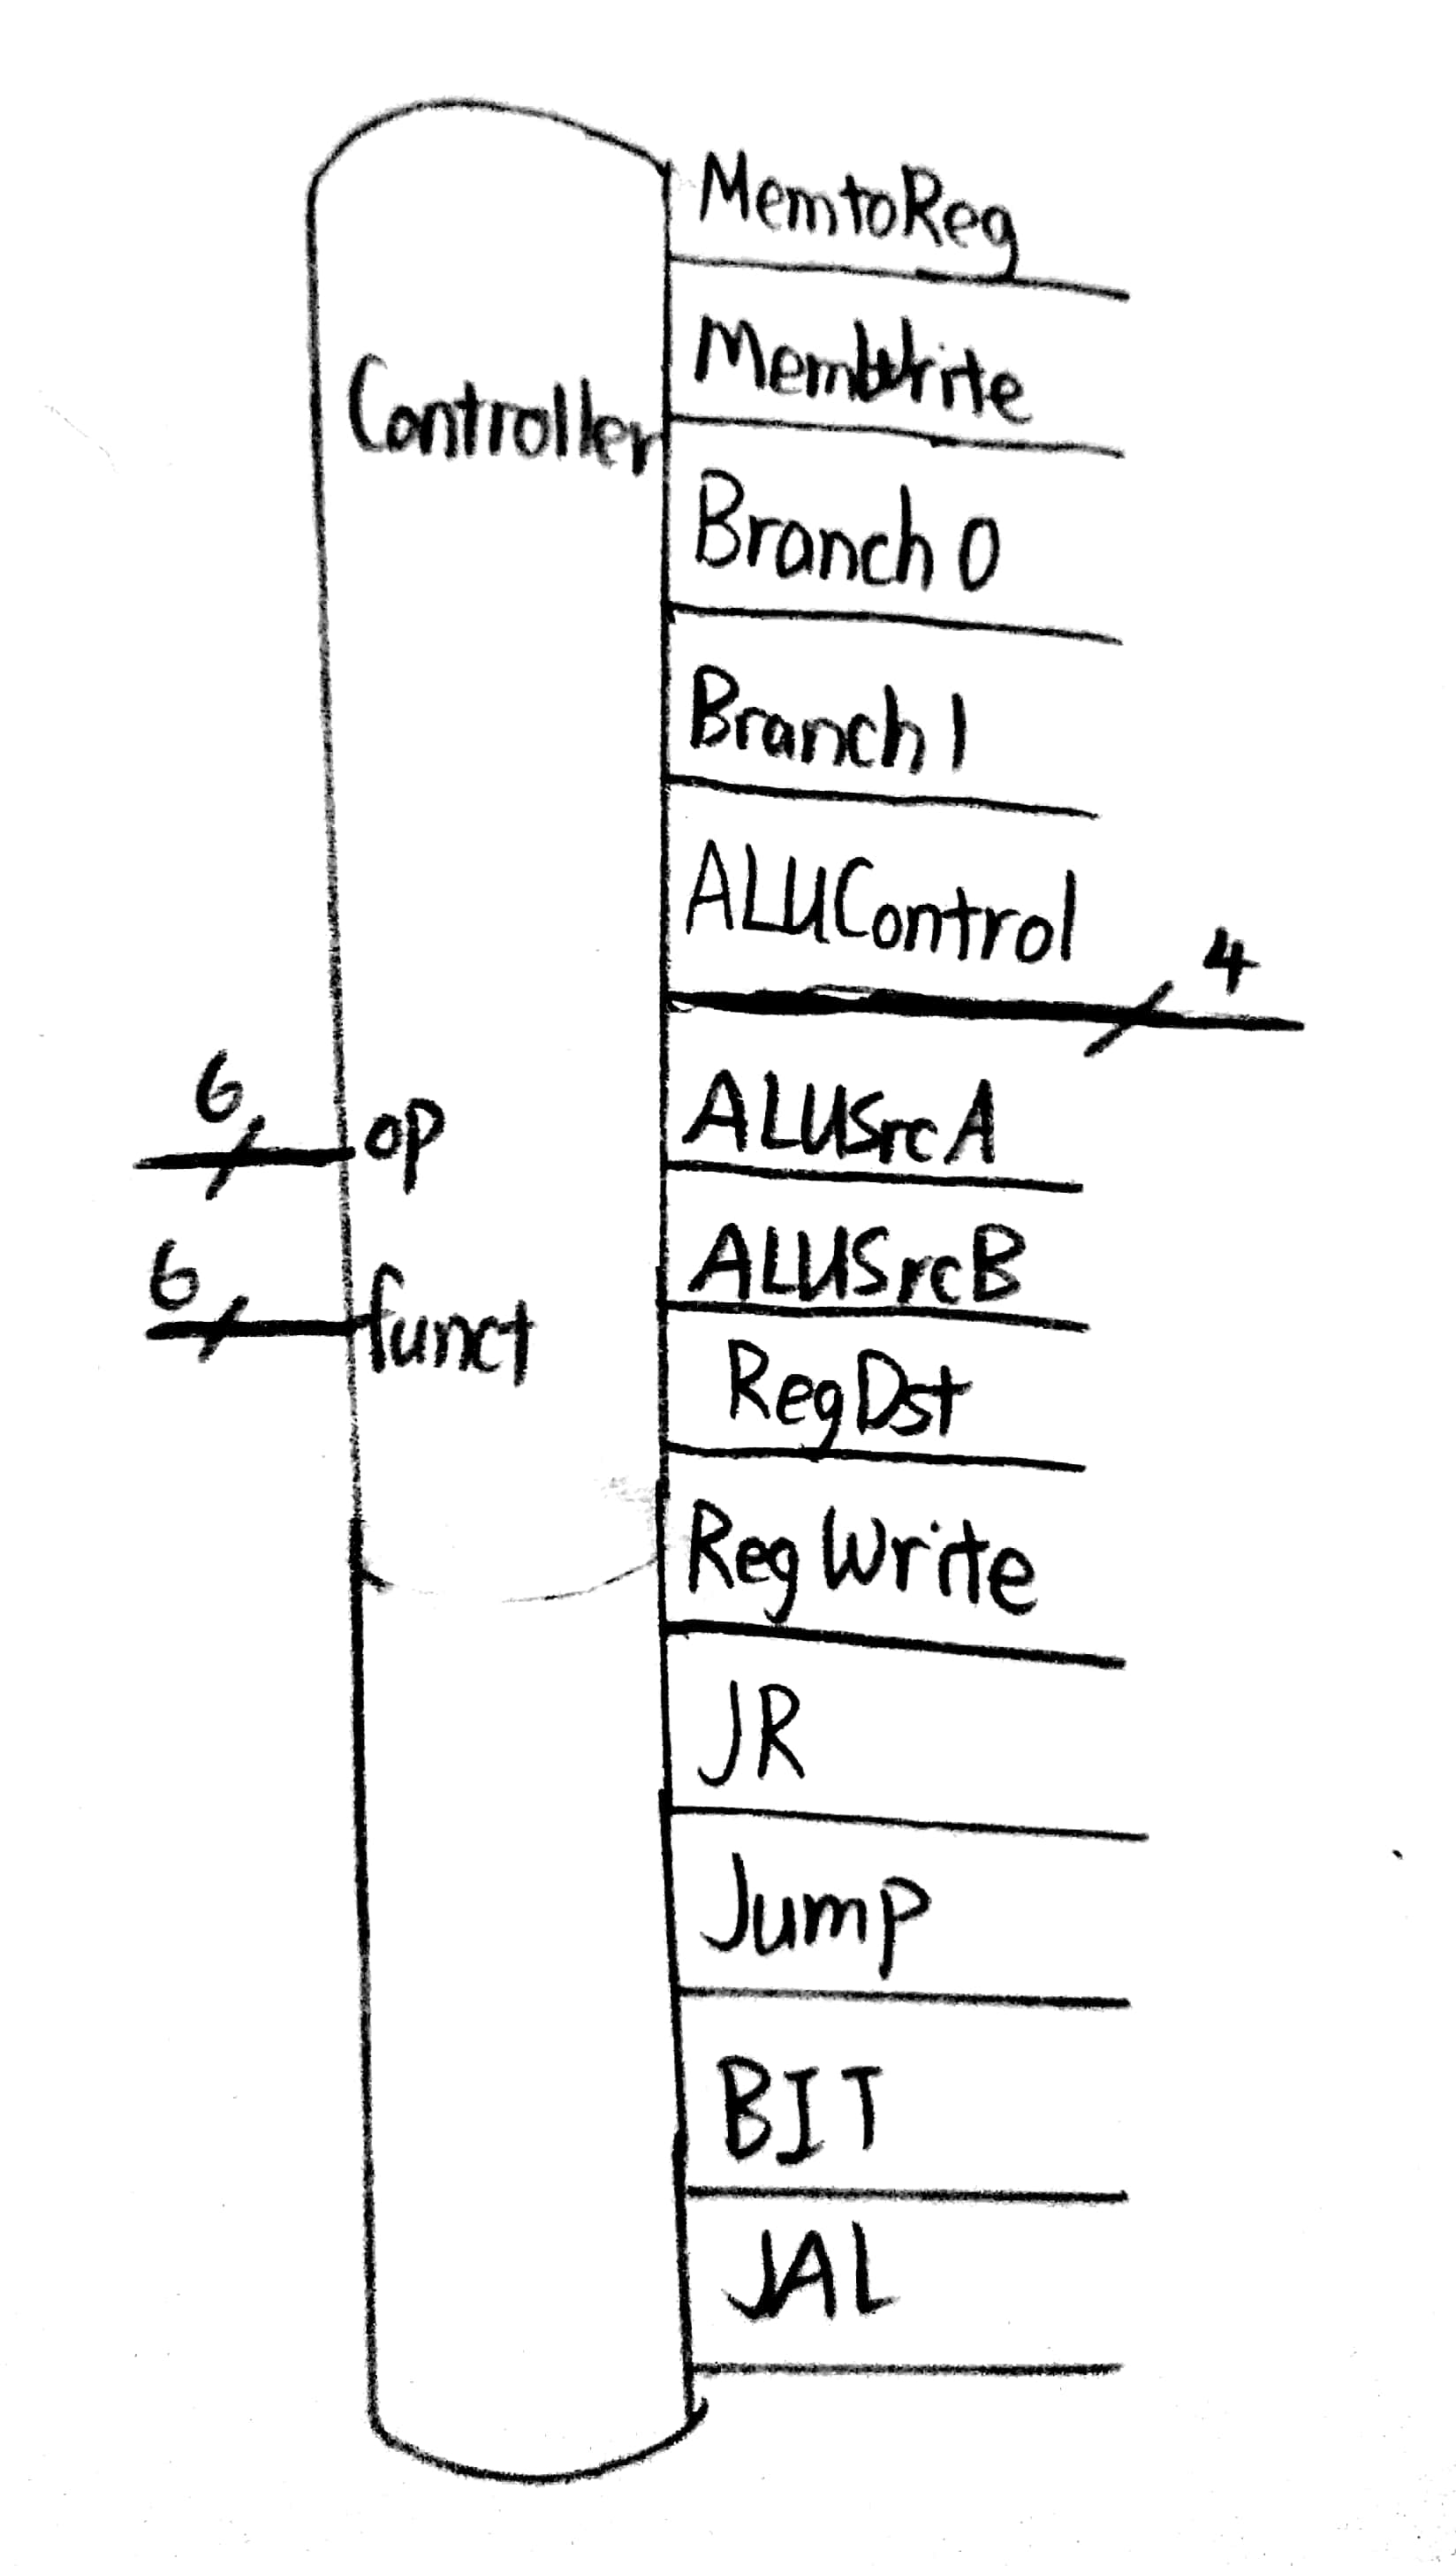
\includegraphics[width =0.3 \linewidth]{figure/Controller.jpg}

{\bf 功能说明:} 根据指令码分配控制信号,详见表~\ref{tab:controller}。为减小表格面积,表头均使用缩写,信号全称依次为RegWrite、RegDst、ALUSrcA、ALUSrcB、Branch0、Branch1、MemWrite、MemtoReg、JR、Jump、JAL、BIT、aluop。

\begin{itemize}
\item 对于需要修改寄存器的指令,RegWrite = 1
\item 对于R类型指令,RegDst = 1;对于I类型指令,RegDst = 0
\item 对于移位操作,ALUSrc = 1
\item 对于部分需要立即数计算的I类型指令,ALUSrcB = 1
\item 对于beq指令,Branch0 = 1;对于bne指令,Branch1 = 1
\item 对于需要写内存的sw指令,MemWrite = 1
\item 对于需要将内存读出的值写入寄存器的lw指令,MemtoReg = 1
\item 对于jr指令,JR = 1;对于jal指令,JAL = 1
\item 对于直接跳转的j和jal指令,J = 1
\item 对于需要补0的I类型位运算,BIT = 1
\item 对于R类型指令,aluop = 010,具体操作由funct决定;对于部分I类型指令,选择相应的运算;对于beq和bne指令,需要做减法,设置aluop = 001
\end{itemize}

{\bf 实现细节:} 为了避免冗杂的赋值语句,我们可以先将控制信号压成一个向量,然后直接用向量赋值即可。
\begin{lstlisting}[language=Verilog]  
assign {RegWrite, RegDst, ALUSrcB, Branch0, Branch1, MemWrite, MemtoReg, Jump, aluop, BIT} = controls;
    always @(*)
      case (op)
        6'b000000: controls <= 12'b110000000100;
        6'b001000: controls <= 12'b101000000000;
        6'b001100: controls <= 12'b101000000111;
        6'b001101: controls <= 12'b101000001001;
        6'b001010: controls <= 12'b101000001010;
        6'b101011: controls <= 12'b001001000000;
        6'b100011: controls <= 12'b101000100000;
        6'b000010: controls <= 12'b00000001xxx0;
        6'b000100: controls <= 12'b000100000010;
        6'b000101: controls <= 12'b000010000010;
        6'b000011: controls <= 12'b10000001xxx0;
        default: controls <= 12'bxxxxxxxxxxxx;
      endcase
\end{lstlisting}  

对于一些特殊的信号,只有极少数情况下为1,则可直接特判得到。
\begin{lstlisting}[language=Verilog]  
assign ALUSrcA = (op == 6'b000000) & ((funct == 6'b000000) | (funct == 6'b000011) | (funct == 6'b000010));
assign JR = (op == 6'b000000) & (funct == 6'b001000);
assign JAL = (op == 6'b000011);
\end{lstlisting}  

对于R类型指令通过funct字段,选择ALUControl的信号;否则,根据op字段,分配aluop信号,借此选择ALUControl信号。
\begin{lstlisting}[language=Verilog]  
always @(*)
        case (aluop)
            3'b000: alucontrol <= 3'b010; 
            3'b001: alucontrol <= 3'b110; 
            3'b011: alucontrol <= 3'b000; 
            3'b100: alucontrol <= 3'b001; 
            3'b101: alucontrol <= 3'b111; 
            default: case(funct)
                6'b100000: alucontrol <= 4'b0010; 
                6'b100010: alucontrol <= 4'b0110; 
                6'b100100: alucontrol <= 4'b0000; 
                6'b100101: alucontrol <= 4'b0001; 
                6'b101010: alucontrol <= 4'b0111; 
                6'b000000: alucontrol <= 4'b0011; 
                6'b000010: alucontrol <= 4'b1000; 
                6'b000011: alucontrol <= 4'b1001; 
                default: alucontrol <= 4'bxxxx; 
              endcase
        endcase
\end{lstlisting}  


%\newpage
\section{测试样例与结果}

\subsection{全部指令all.in}

\begin{lstlisting}[]  
 0x0 : addi $s0, $0, 12     | 2010000c
 0x4 : andi $s2, $s0, -8    | 3212fff8
 0x8 : ori $s3, $s1, 10     | 3633000a
 0xc : slti $s4, $s2, 5     | 2a540005
0x10 : nop                  | 00000000
0x10 : add $t0, $s0, $s1    | 02114020
0x14 : sub $t0, $s2, $s3    | 02534022
0x18 : and $t0, $s3, $s1    | 02714024
0x1c : or $t0, $s1, $s2     | 02324025
0x20 : slt $t0, $s0, $s2    | 0212402a
0x24 : sw $s0, 2($0)        | ac100002
0x28 : lw $t0, 2($0)        | 8c080002
\end{lstlisting}  

\subsection{位运算测试test\_sign.in}

\begin{lstlisting}[]  
 0x0 : addi $s0, $0, 0xffff | 2010ffff
 0x4 : add $s0, $s0, $s0    | 02108020
 0x8 : andi $t0, $s0, 0xffff | 3208ffff
\end{lstlisting}  

\subsection{条件跳转condition\_beq.in}

\begin{lstlisting}[]  
 0x0 : addi $s0, $0, 4      | 20100004
 0x4 : addi $s1, $0, 1      | 20110001
 0x8 : addi $s1, $s1, 3     | 22310003
 0xc : beq $s0, $s1, target | 12300002
0x10 : addi $s1, $s1, 1     | 22310001
0x14 : sub $s1, $s1, $s0    | 02308822
0x18 :                      | 
0x18 : target:              | 
0x18 : add $s1, $s1, $s0    | 02308820
\end{lstlisting}  

\subsection{switch语句switch.in}

\begin{lstlisting}[]  
 0x0 : addi $s0, $0, 100    | 20100064
 0x4 :                      | 
 0x4 : case20:              | 
 0x4 : addi $t0, $0, 20     | 20080014
 0x8 : bne $s0, $t0, case50 | 15100002
 0xc : addi $s1, $0, 2      | 20110002
0x10 : j done               | 0800000e
0x14 : case50:              | 
0x14 : addi $t0, $0, 50     | 20080032
0x18 : bne $s0, $t0, case100 | 15100002
0x1c : addi $s1, $0, 3      | 20110003
0x20 : j done               | 0800000e
0x24 : case100:             | 
0x24 : addi $t0, $0, 100    | 20080064
0x28 : bne $s0, $t0, default | 15100002
0x2c : addi $s1, $0, 5      | 20110005
0x30 : j done               | 0800000e
0x34 : default:             | 
0x34 : add $s1, $0, $0      | 00008820
0x38 :                      | 
0x38 : done:                | 
\end{lstlisting}  

\subsection{while循环while\_loop.in}

\begin{lstlisting}[]  
 0x0 : addi $s0, $0, 1      | 20100001
 0x4 : addi $s1, $0, 0      | 20110000
 0x8 :                      | 
 0x8 : addi $t0, $0, 128    | 20080080
 0xc : while:               | 
 0xc : beq $s0, $t0, done   | 11100003
0x10 : add $s0, $s0, $s0    | 02108020
0x14 : addi $s1, $s1, 1     | 22310001
0x18 : j while              | 08000003
0x1c : done:                | 
\end{lstlisting}  

\subsection{for循环for\_loop.in}

\begin{lstlisting}[]   
 0x0 : add $s1, $0, $0      | 00008820
 0x4 : addi $s0, $0, 0      | 20100000
 0x8 : addi $t0, $0, 10     | 2008000a
 0xc :                      | 
 0xc : for:                 | 
 0xc : beq $s0, $t0, done   | 11100003
0x10 : add $s1, $s1, $s0    | 02308820
0x14 : addi $s0, $s0, 1     | 22100001
0x18 : j for                | 08000003
0x1c :                      | 
0x1c : done:                | 
\end{lstlisting}  

\subsection{{\color{red} 快速乘法quick\_multiply.in}}

\begin{lstlisting}[]  
 0x0 : addi $t0, $0, 99     | 20080063
 0x4 : addi $t1, $0, 37     | 20090025
 0x8 : addi $s0, $0, 0      | 20100000
 0xc :                      | 
 0xc : while:               | 
 0xc : beq $t1, $0, done    | 10090006
0x10 : andi $t2, $t1, 1     | 312a0001
0x14 : beq $t2, $0, target  | 100a0001
0x18 : add $s0, $s0, $t0    | 02088020
0x1c : target:              | 
0x1c : sll $t0, $t0, 1      | 00084040
0x20 : srl $t1, $t1, 1      | 00094842
0x24 : j while              | 08000003
0x28 :                      | 
0x28 : done:                | 
\end{lstlisting}  

\subsection{{\color{red} 递归测试factorial.in}}

\begin{lstlisting}[]  
 0x0 : addi $sp, $0, 128    | 201d0080
 0x4 : addi $a0, $0, 5      | 20040005
 0x8 : jal factorial        | 0c000004
 0xc : sll $v0, $v0, 1      | 00021040
0x10 :                      | 
0x10 : factorial:           | 
0x10 : addi $sp, $sp, -8    | 23bdfff8
0x14 : sw $a0, 4($sp)       | afa40004
0x18 : sw $ra, 0($sp)       | afbf0000
0x1c : addi $t0, $0, 2      | 20080002
0x20 : slt $t0, $a0, $t0    | 0088402a
0x24 : beq $t0, $0 ,else    | 10080003
0x28 : addi $v0, $0, 1      | 20020001
0x2c : addi $sp, $sp, 8     | 23bd0008
0x30 : jr $ra               | 03e00008
0x34 : else:                | 
0x34 : addi $a0, $a0, -1    | 2084ffff
0x38 : jal factorial        | 0c000004
0x3c : lw $ra, 0($sp)       | 8fbf0000
0x40 : lw $a0, 4($sp)       | 8fa40004
0x44 : addi $sp, $sp, 8     | 23bd0008
0x48 : add $v0, $a0, $v0    | 00821020
0x4c : jr $ra               | 03e00008
\end{lstlisting}  

\newpage
\section{讨论}

\subsection{显示寄存器选择}

\subsection{时钟频率调节}

\subsection{显示模块Display}

\section{注意事项}

\begin{enumerate}
\item Run Implementation前必须先写好xdc文件,并且顶层模块要有输出口。
\item always模块中只能对reg类型的变量赋值。
\item 读逻辑要写成组合逻辑,否则写入时不能同步内存中的值。
\end{enumerate}

\end{sloppypar}
\end{document}
